\documentclass[a4paper, 12pt]{article}
\usepackage[utf8]{inputenc}
\usepackage[slovene]{babel}

\usepackage{amsthm}
\usepackage{amsmath, amssymb, amsfonts}
\usepackage{relsize}
\usepackage{graphicx}
\usepackage{etoolbox}
\usepackage{setspace}
\graphicspath{ {./Slike/} }
\usepackage[
top    = 2.5cm,
bottom = 3.cm,
left   = 2.5cm,
right  = 2.5cm]{geometry}
\usepackage{hyperref}
\usepackage{mathtools}
\usepackage{authblk}
\usepackage{makecell}
\usepackage[nottoc]{tocbibind}
\usepackage{algorithm}
\usepackage[noend]{algpseudocode}
\usepackage{listings}
\usepackage{mathabx}
\floatname{algorithm}{Algoritem}
\renewcommand{\listalgorithmname}{Kazalo algoritmov}
\algnewcommand\algorithmicto{\textbf{to}}
\algnewcommand\algorithmicin{\textbf{in}}
\algnewcommand\algorithmicforeach{\textbf{for each}}
\algrenewtext{For}[3]{\algorithmicfor\ #1 $\gets$ #2\ \algorithmicto\ #3\ \algorithmicdo}
\algdef{S}[FOR]{ForEach}[2]{\algorithmicforeach\ #1\ \algorithmicin\ #2\ \algorithmicdo}

\makeatletter
\def\BState{\State\hskip-\ALG@thistlm}
\makeatother


\newtheorem{definicija}{Definicija}
\newtheorem{posledica}{Posledica}

\begin{document}

\begin{titlepage}
    \begin{center}
        \textsc{\LARGE Univerza v Ljubljani}\\[0.5cm]
        {\Large Fakulteta za matematiko in fiziko}\\[3cm]
        {\large Finančni praktikum}\\[0.5cm]
        {\huge Največje neodvisne množice z lokalnim iskanjem}\\[10.0cm]
    \end{center}

    \begin{minipage}{0.4\textwidth}
		\begin{flushleft}
			\large
			\textit{Avtorja:}\\
			Jaka Mrak \\
			Žiga Gartner 
		\end{flushleft}
	\end{minipage}
	~
	\begin{minipage}{0.4\textwidth}
		\begin{flushright}
			\large
			\textit{Mentorja:}\\
			prof. dr. Sergio \textsc{Cabello} \\
			doc. dr. Janoš \textsc{Vidali}
		\end{flushright}
	\end{minipage}
	
	\vfill\vfill\vfill 
	\begin{center}
	{\large{Ljubljana, \today}} 
    \end{center}
	\vfill 

\end{titlepage}

\tableofcontents
\listoffigures

\newpage

\section{Navodilo}

Naloga je iskanje največje neodvisne množice v grafu $G = (V,E)$ s pomočjo celoštevilskega linearnega programiranja. Velike neodvisne množice v grafu lahko poiščemo s pomočjo metode lokalnega iskanja.
Začnemo s poljubno neodvisno množico $U  \subseteq V$, kjer $k$ vozlišč nadomestimo s $k + 1$ vozlišči tako, da ohranjamo neodvisnost množice $U$. Konstanta $k$ je dana na začetku. Primerjali bomo metodi
lokalnega iskanja in optimalne rešitve ter primerjali njune rešitve za nekatere preproste grafe.

\section{Opis problema}
\begin{definicija}
    Naj bo $G = (V,E)$ graf. \textbf{Neodvisna množica} $U$, v grafu $G$, je taka podmnožica množice vozlišč $V$, kjer poljubni dve vozlišči iz množice $U$ nista sosednji.
    \textbf{Maksimalna neodvisna množica} v grafu $G$ pa je taka neodvisna množica, kjer ne obstaja vozlišče $v \in V$ in $v \notin U$, ki bi ga lahko dodali množici $U$ in pri tem ohranili neodvisnost množice $U$. Torej
    je neodvisna množica $U$ največja taka, če velja ena od naslednjih dveh lastnosti:
    \begin{enumerate}
        \item $v \in U$
        \item $S(v) \cap U \neq \emptyset,$ kjer je $S(v)$ množica sosedov $v$.
    \end{enumerate}
    \textbf{Največja neodvisna množica} je neodvisna množica, največje možne velikosti, za dan graf $G$. Velikosti največje neodvisne množice, za graf $G$, pa pravimo \textbf{neodvisnostno število} in 
    pogosto označimo $\alpha(G)$.
\end{definicija}

\begin{definicija}
    Celoštevilski linearni program v standardni obliki je dan z matriko $A \in \mathbb{R}^{m \times n}$, vektorjem $b \in \mathbb{R}^{m}$ in vektorjem $c \in \mathbb{R}^{n}$. Iščemo
    $$max<c,x>,$$
    da bodo zadoščeni pogoji
    $$ Ax \leq b, x \geq 0,$$
    kjer je $x \in \mathbb{Z}^{n}.$

\end{definicija}

\begin{posledica}
Problem največje neodvisne množice v grafu $G=(V,E)$ lahko s celoštevilskim linearnim programiranjem modeliramo na sledeč način:
$$max \sum_{v \in V} x_{v},$$
da velja:
$$ x_{v} + x_{w} \leq 1 \ za \ \forall vw \in E,$$
$$ x_{v} \in \{0, 1 \}$$
$$ x_{u} = 
    \begin{cases}
    1, \ za \ u \in U \\
    0, \ za \ u \notin U
    \end{cases}, \text{U neodvisna množica v grafu G.}
$$
\end{posledica}

\noindent Največjo neodvisno množico v množici vseh neodvisnih podmnožic grafa $G = (V,E)$ bomo iskali s pomočjo celoštevilskega lineranega programiranja in lokalnega iskanja. \textbf{Lokalno iskanje} temelji na
izbiri začetne neodvisne podmnožiče vozlišč $U \subset V$ v kateri $k$ vozlišč zamenjamo s $k + 1$ vozlišči in pri tem ohranjamo neodvisnost množice $U$.

\newpage

\section{Opis dela}
V nadaljevanju bomo največjo/maksimalne neodvisne množice iskali s pomočjo $CLP$ v Sage in s pomočjo implementiranega algoritma $nakljucni\_MIS(G)$,  kasneje izboljšanega z lokalnim
iskanjem. Algoritme bomo izvajali na grafih, generiranih s pomočjo \\
$\text{Erdős-Rényijevega}\ G(n,p)$ modela. Primerjali bomo maksimalne (ali pa največje) neodvisne množice, ki jih algoritmi poiščejo,
časovno zahtevnost algoritmov, kasneje pa še, kako vpliva spreminjanje števila vozlišč in verjetnosti, v modelu, na velikost maksimalne (ali pa največje) neodvisne množice in na
časovno zahtevnost algoritmov.

\subsection{Generiranje podatkov}
Kot omenjeno, bomo grafe generirali s pomočjo $\text{Erdős-Rényijevega}\ G(n,p)$ modela, kjer podamo algoritmu parameter $n$ za število vozlišč in $p$ za verjetnost, da sta poljubni vozlišči povezani.

\begin{definicija}
    $\text{Erdős-Rényijev}$ model $G(n, p)$ generira graf z $n$ naključno povezanimi vozlišči. Vsaka povezava je v graf vključena neodvisno, z verjetnostjo $p$.
\end{definicija}

\noindent Generirali bomo grafe s spreminjajočima vrednostma $(n,p)$. Najprej z naraščajočim $n$ in konstantnim $p$, nato pa še s konstantim $n$ in naraščajočim $p$. Za generacijo podatkov v Pythonu bomo uporabili
knjižnico $NetworkX$. Da bomo lahko grafe uporabljali še v okolju $Sage$, bomo le-te s funkcijo $nx.to\_dict\_of\_lists(graf)$, kjer je $nx$ okrajšava za $NetworkX$, pretvorili v slovarje seznamov.
Grafe, na katerih bomo izvajali algoritme, bomo shranili v $JSON$ datoteke, da imamo evidenco na kakšnih grafih smo izvajali algoritme.


\subsection{Algoritmi}

Za iskanje maksimalne neodvisne množice smo implementirali algoritem $nakljucni\_MIS(G)$, čigar rešitev bomo poizkušali izboljšati še z algoritmom $lokalno\_iskanje(G, I)$. Oba
algoritma bosta kot argument sprejela graf $G$, algoritem $lokalno\_iskanje(G, I)$ pa še neko maksimalno neodvisno množico $I$ grafa $G$.

\subsubsection{Algoritem \textbf{$nakljucni\_MIS(G)$}}

\begin{algorithm}
\caption{$nakljucni\_MIS(G)$}\label{euclid}
\begin{algorithmic}[1]
\State $\textit{I} = \emptyset$
\State $\forall v \in V\ \text{dobi vrednost}\ \textit{P}(v) \in \textit{permutacija}(V)$
\If {$\textit{P}(v) < \textit{P}(w)\ \textit{za}\ \forall w \in \textit{sosedi}(v) $}
\State $ I = I \cup v $
\EndIf
\State $V' = V \setminus (I \cup \textit{sosedi}(I))$.
\State $E' = E \setminus \textit{povezave}(I)$.
\State $\text{return}\  I \cup \textit{MIS}(G'=(V', E'))$
\end{algorithmic}
\end{algorithm}

\newpage

\subsubsection{Algoritem $lokalno\_iskanje(G, I)$}

Najprej definirajmo $\tau(v)$, v algoritmu imenovan $tightness(v)$.
\begin{definicija}
	Naj bo $G=(V,E)$ in $v \in S \subset G$. Potem je:
	$$\tau(v) = |W|, \ kjer \ je \ W = \{w|w \in (sosedi(v) \cap V \setminus S)\}.$$
\end{definicija}

\noindent Algoritem $lokalno\_iskanje(G, I)$ sprejme graf $G$ in neko maksimalno neodvisno množico v grafu $G$. Nato vsakemu vozliscu $v \in I$
priredi mnozico $L(v) = \{w \in sosedi(v)| \tau(w) = 1\}$. Če je ta množica več kot, ali pa dvo elementna, potem v vseh možnih parih 
$(x, y) \in L(v) \bigtimes L(v)$, ki zadoščajo $x \neq y$, poišče prvega, da velja $y \notin sosedi(x)$, ko najde prvi tak par iz množice $I$
odstrani vozlišče $v$, in množici $I$ doda vozlišči $x$ in $y$. Algoritem vrne maksimalno neodvisno množico $I$, ko ne obstaja $z \in I$,
da bi veljalo $|L(z)| \geq 2$.

\begin{lstlisting}[language=Python, basicstyle=\tiny]
import networkx as nx

def tightness(graf, mnozica, v): 
    t = 0
    for w in graf.neighbors(v):
        if w in mnozica:
            t += 1
        else:
            pass
    return t

def lokalno_iskanje(G, I): 
    V = list(G.nodes)
    for v in I:
        L = [] 
        for w in G.neighbors(v):
            if G.neighbors(v) != []:
                if tightness(G, I, w) == 1:
                    L.append(w)
                else:
                    pass
            else:
                pass
        while len(L) >= 2:
            for v1 in L:
                L.remove(v1)
                for w1 in L:
                    if w1 not in G.neighbors(v1):
                        I.remove(v)
                        I = I + [v1, w1]
                        break
                    elif w1 in G.neighbors(v1):
                        pass
                if w1 not in G.neighbors(v1):
                    break
            if w1 not in G.neighbors(v1):
                break
    return I
\end{lstlisting}

\subsection{Analiza rezultatov}

\subsubsection{Analiza algoritmov na grafih $G(50, 0.3)$}

Najprej bomo primerjali algoritme na $\text{Erdős-Rényijevih}\ G(50, 0.3)$. Na tak način sva generirala 500 grafov in na njih izvedla algoritma $CLP(G)$, $nakljucni\_MIS(G)$, za vsak graf pa sva slednjega poskušala izboljšati
še z algoritmom $lokalno\_iskanje(G, I)$, ki poleg grafa $G$ sprejme še $I = nakljucni\_MIS(G)$.\\

\noindent Opazimo, da neodvisne množice največjih moči najde $CLP$. Variacije moči neodvisnih množic,
ki jih lahko vidimo na spodnjem grafu, so rezultat naključnosti pri generiranju $G(50, 0.3)$ grafov.
Od slučaja je namreč odvisno, kako bodo postavljene povezave v grafu $G$.


\begin{figure}[h!]
	\begin{center}
		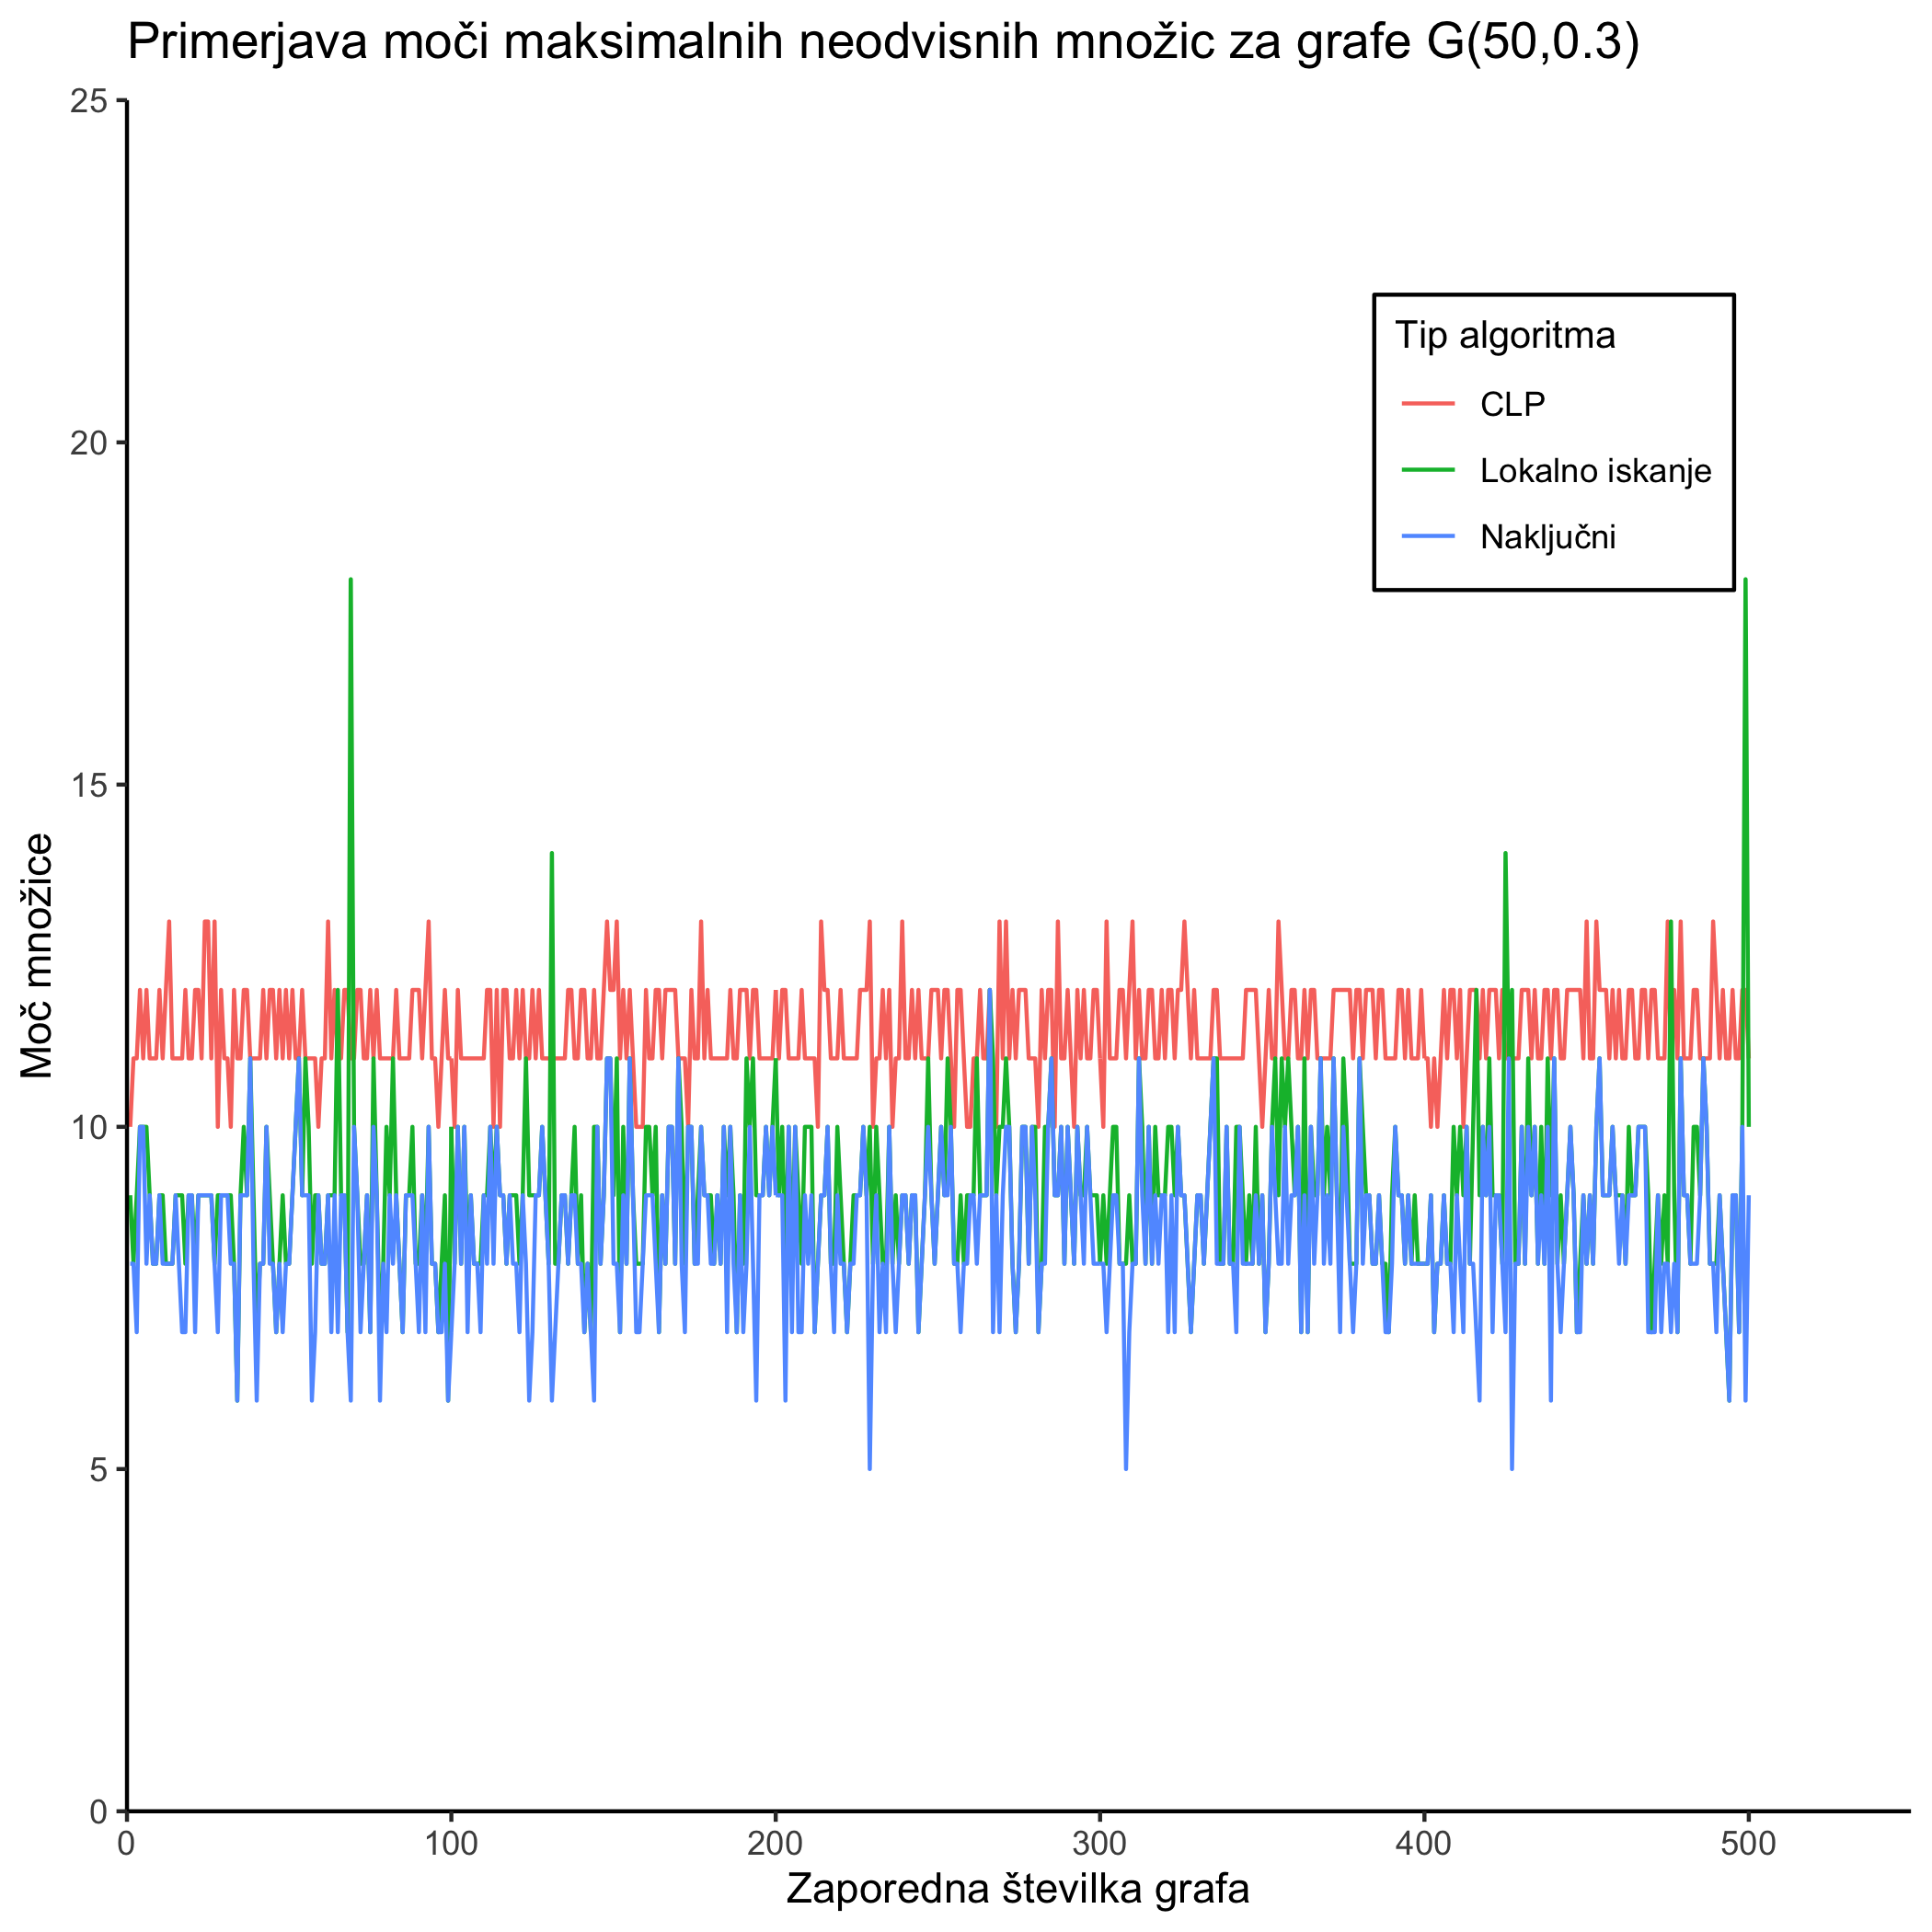
\includegraphics[scale=0.11]{R_koda/pon-moc.png}
		\caption{Moči neodvisnih množic za grafe $G(50,0.3)$}
	\end{center}
\end{figure}

\noindent Kljub temu, da je, za generirane grafe, $CLP$ najpogosteje vrnil najboljšo rešitev, lahko v naslednjem grafu vidimo njegovo slabost. $CLP$ je namreč občutno počasnejši od preostalih dveh algoritmov. 


\begin{figure}[h!]
	\begin{center}
		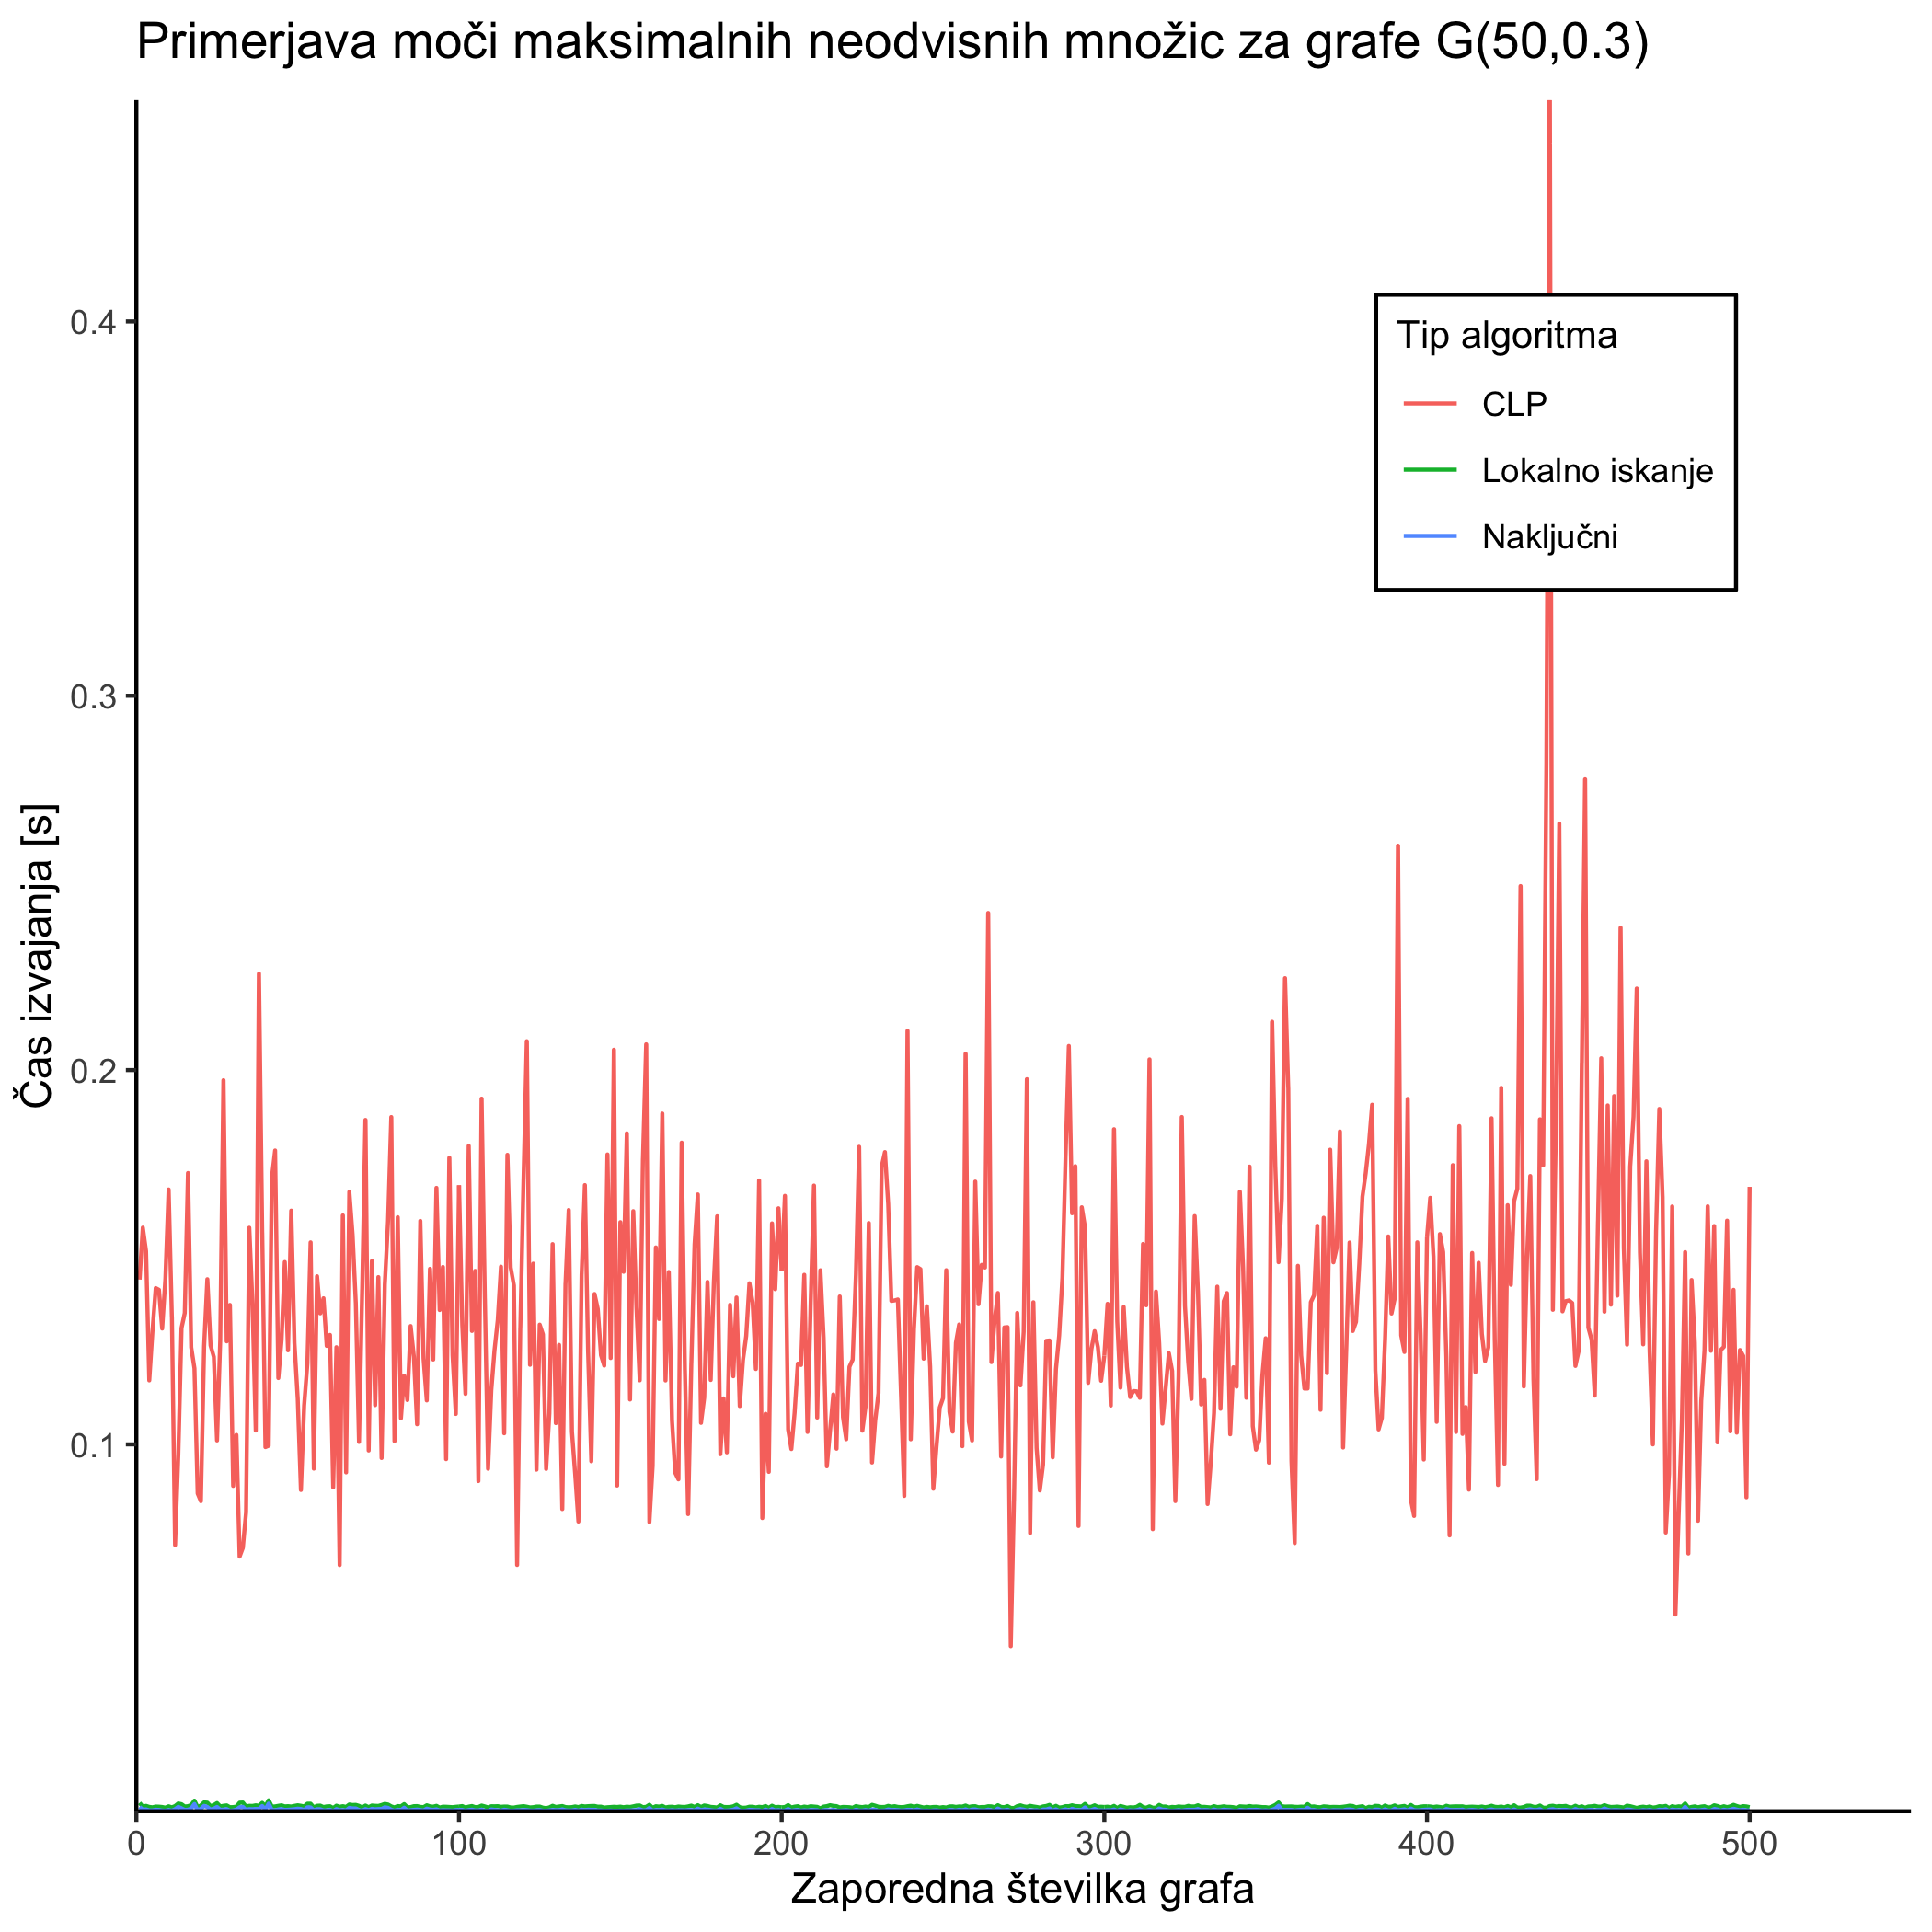
\includegraphics[scale=0.11]{R_koda/pon-casi.png}
		\caption{Časovne zahtevnosti algoritmov za $G(50, 0.3)$}
	\end{center}
\end{figure}

\noindent Poglejmo si sedaj še odstopanja rešitev \textit{lokalnega\_iskanja} od rešitev dobljenih s $CLP$. Hitro pazimo, da je odstopanje nekako \textit{"normalno"} porazdeljeno. Neodvisna množica dobljena z  $lokalnim\ iskanjem$ največkrat odstopa za dve vozlišči od tiste dobljene s $CLP$, 
v nekaj primerih se ti popolnoma ujemata, zelo redko pa se razlikujeta za 4 ali 5 vozlišč.

\begin{figure}[h!]
	\begin{center}
		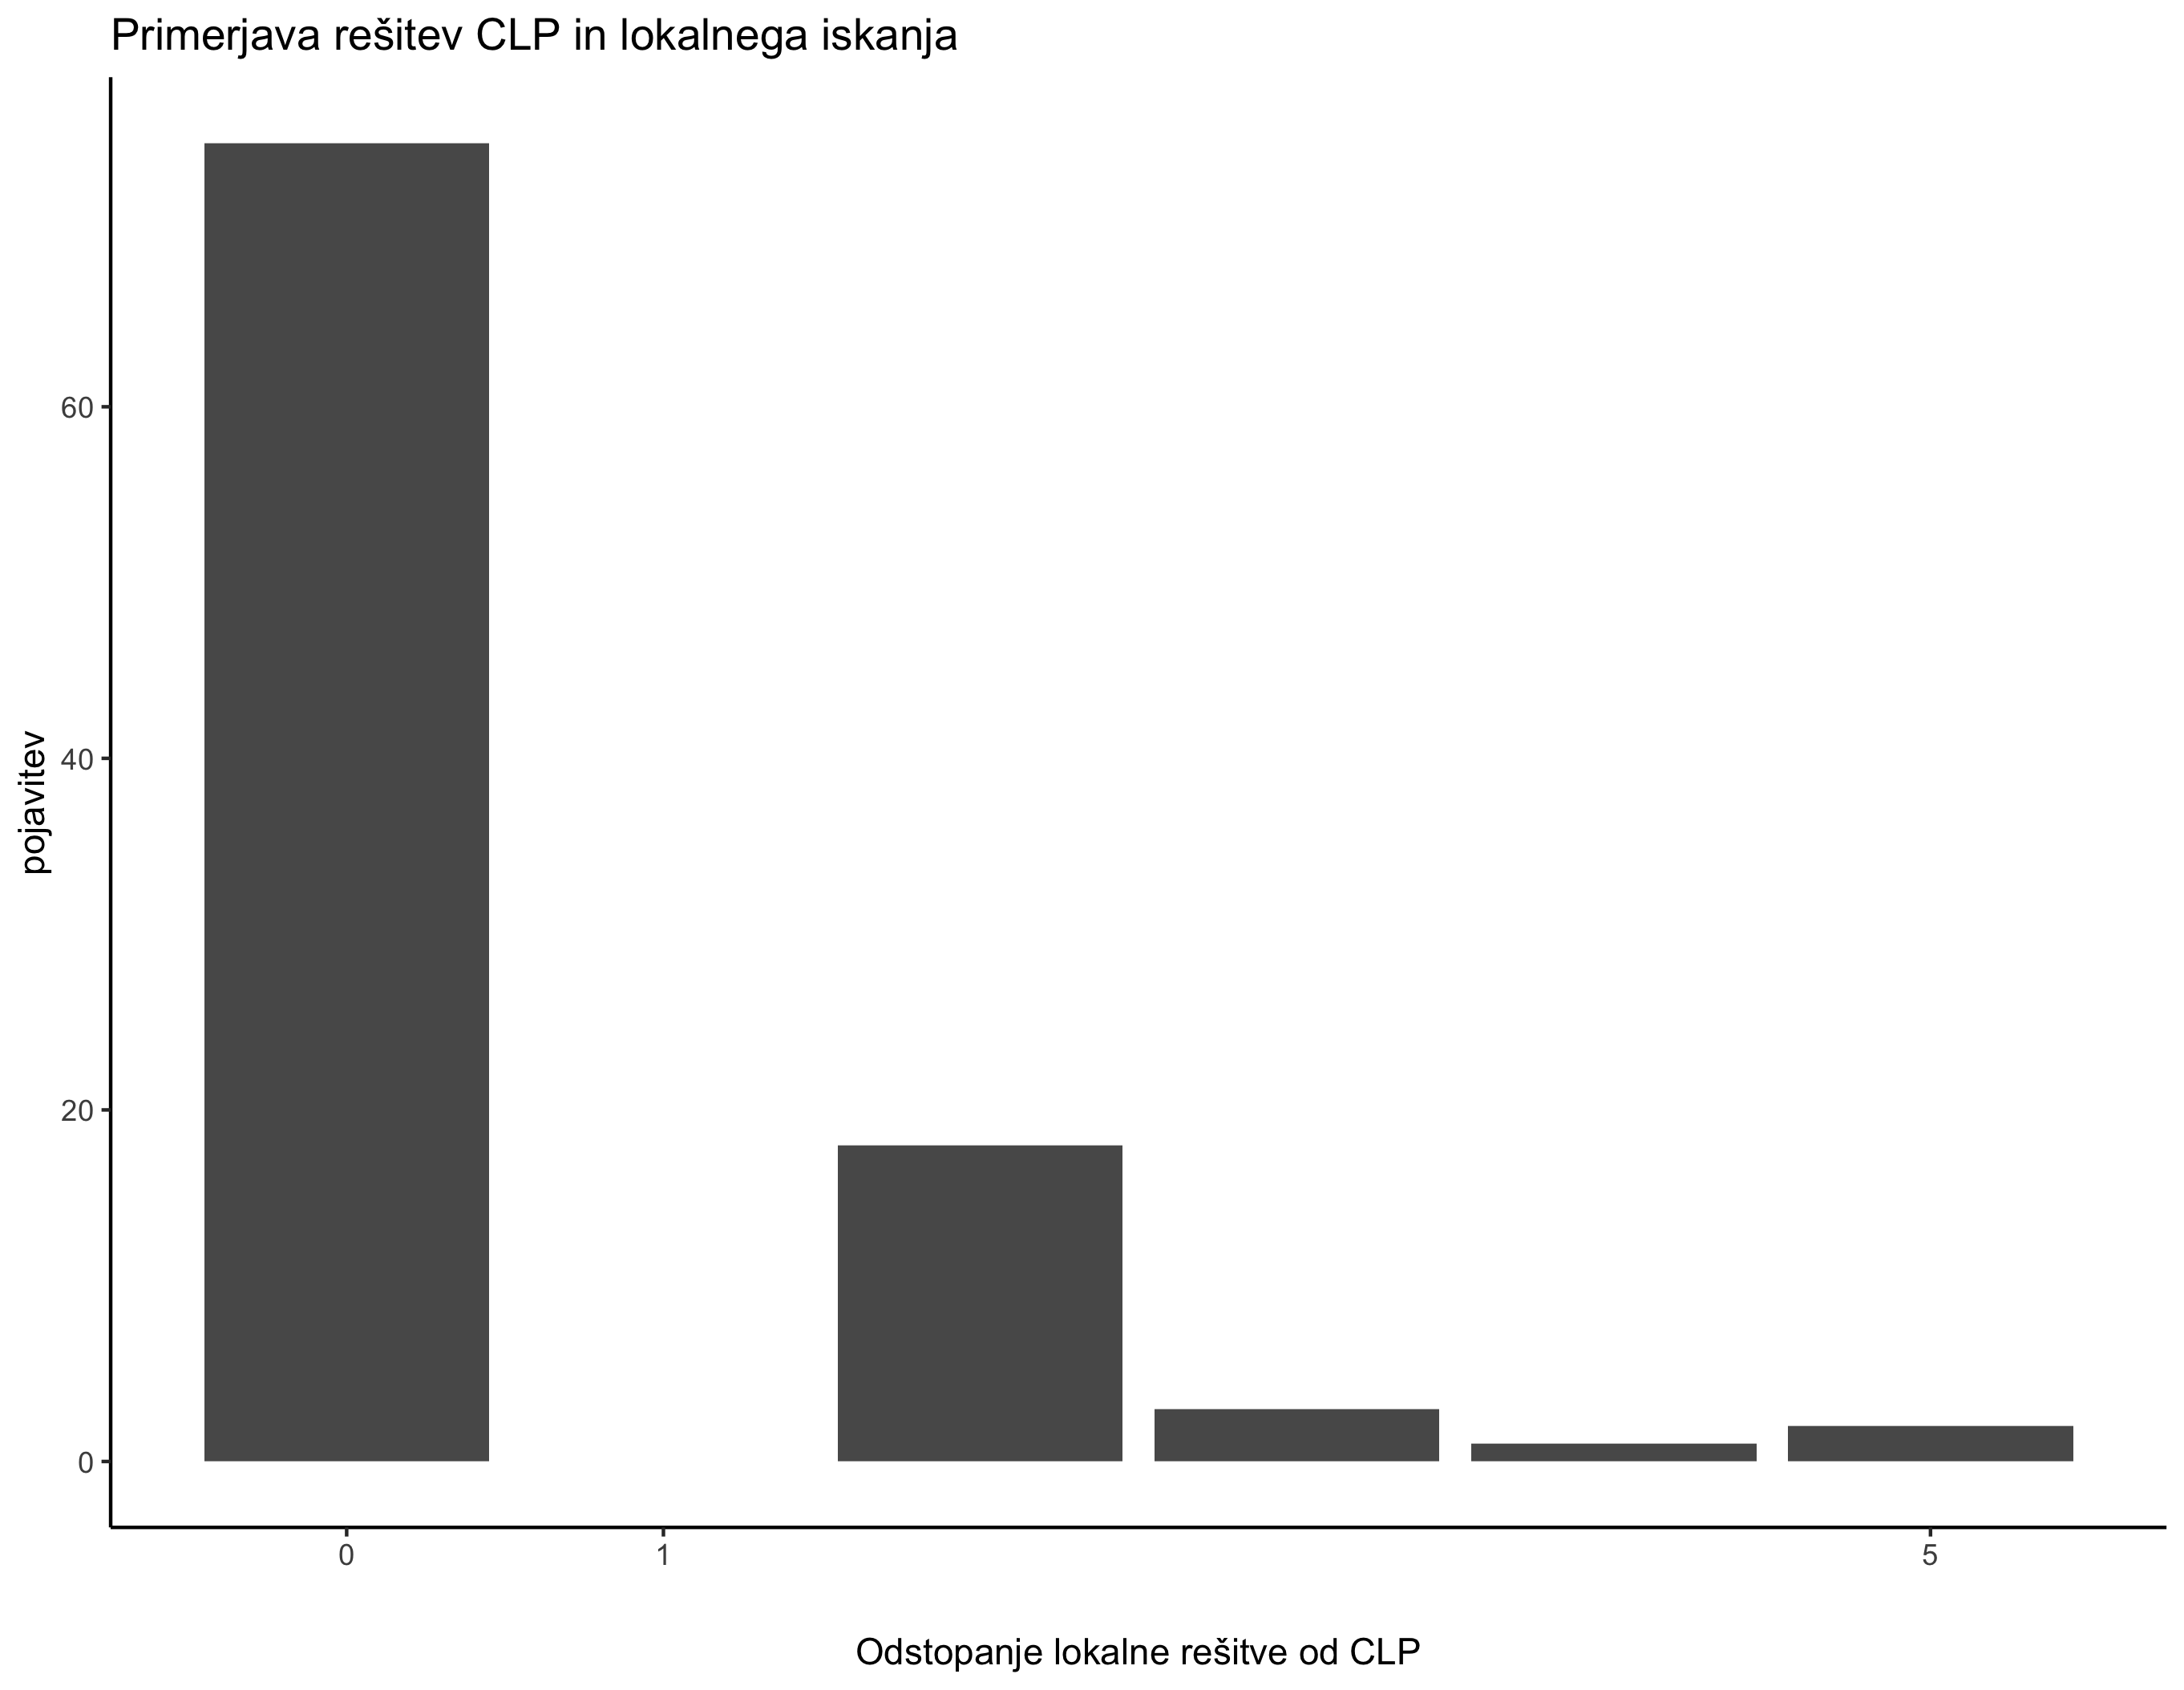
\includegraphics[scale=0.11]{R_koda/pon-napake.png}
		\caption{Odstopanja rešitev lokalnega iskanja do CLP.}
	\end{center}
\end{figure}

\noindent Kot omenjeno, je maksimalne neodvisne množice z najvišjimi močmi vračal $CLP$, s povprečno močjo največje neodvisne množice 12. Druge največje množice je vračalo $lokalno\_iskanje$,
katerega množice so imele v povprečju 9 vozlišč, za eno več od povprečja moči neodvisnih množic najdenih z algoritmom $nakljucni\_MIS$. Rezultati so vidni na spodnjem grafu.

\begin{figure}[h!]
	\begin{center}
		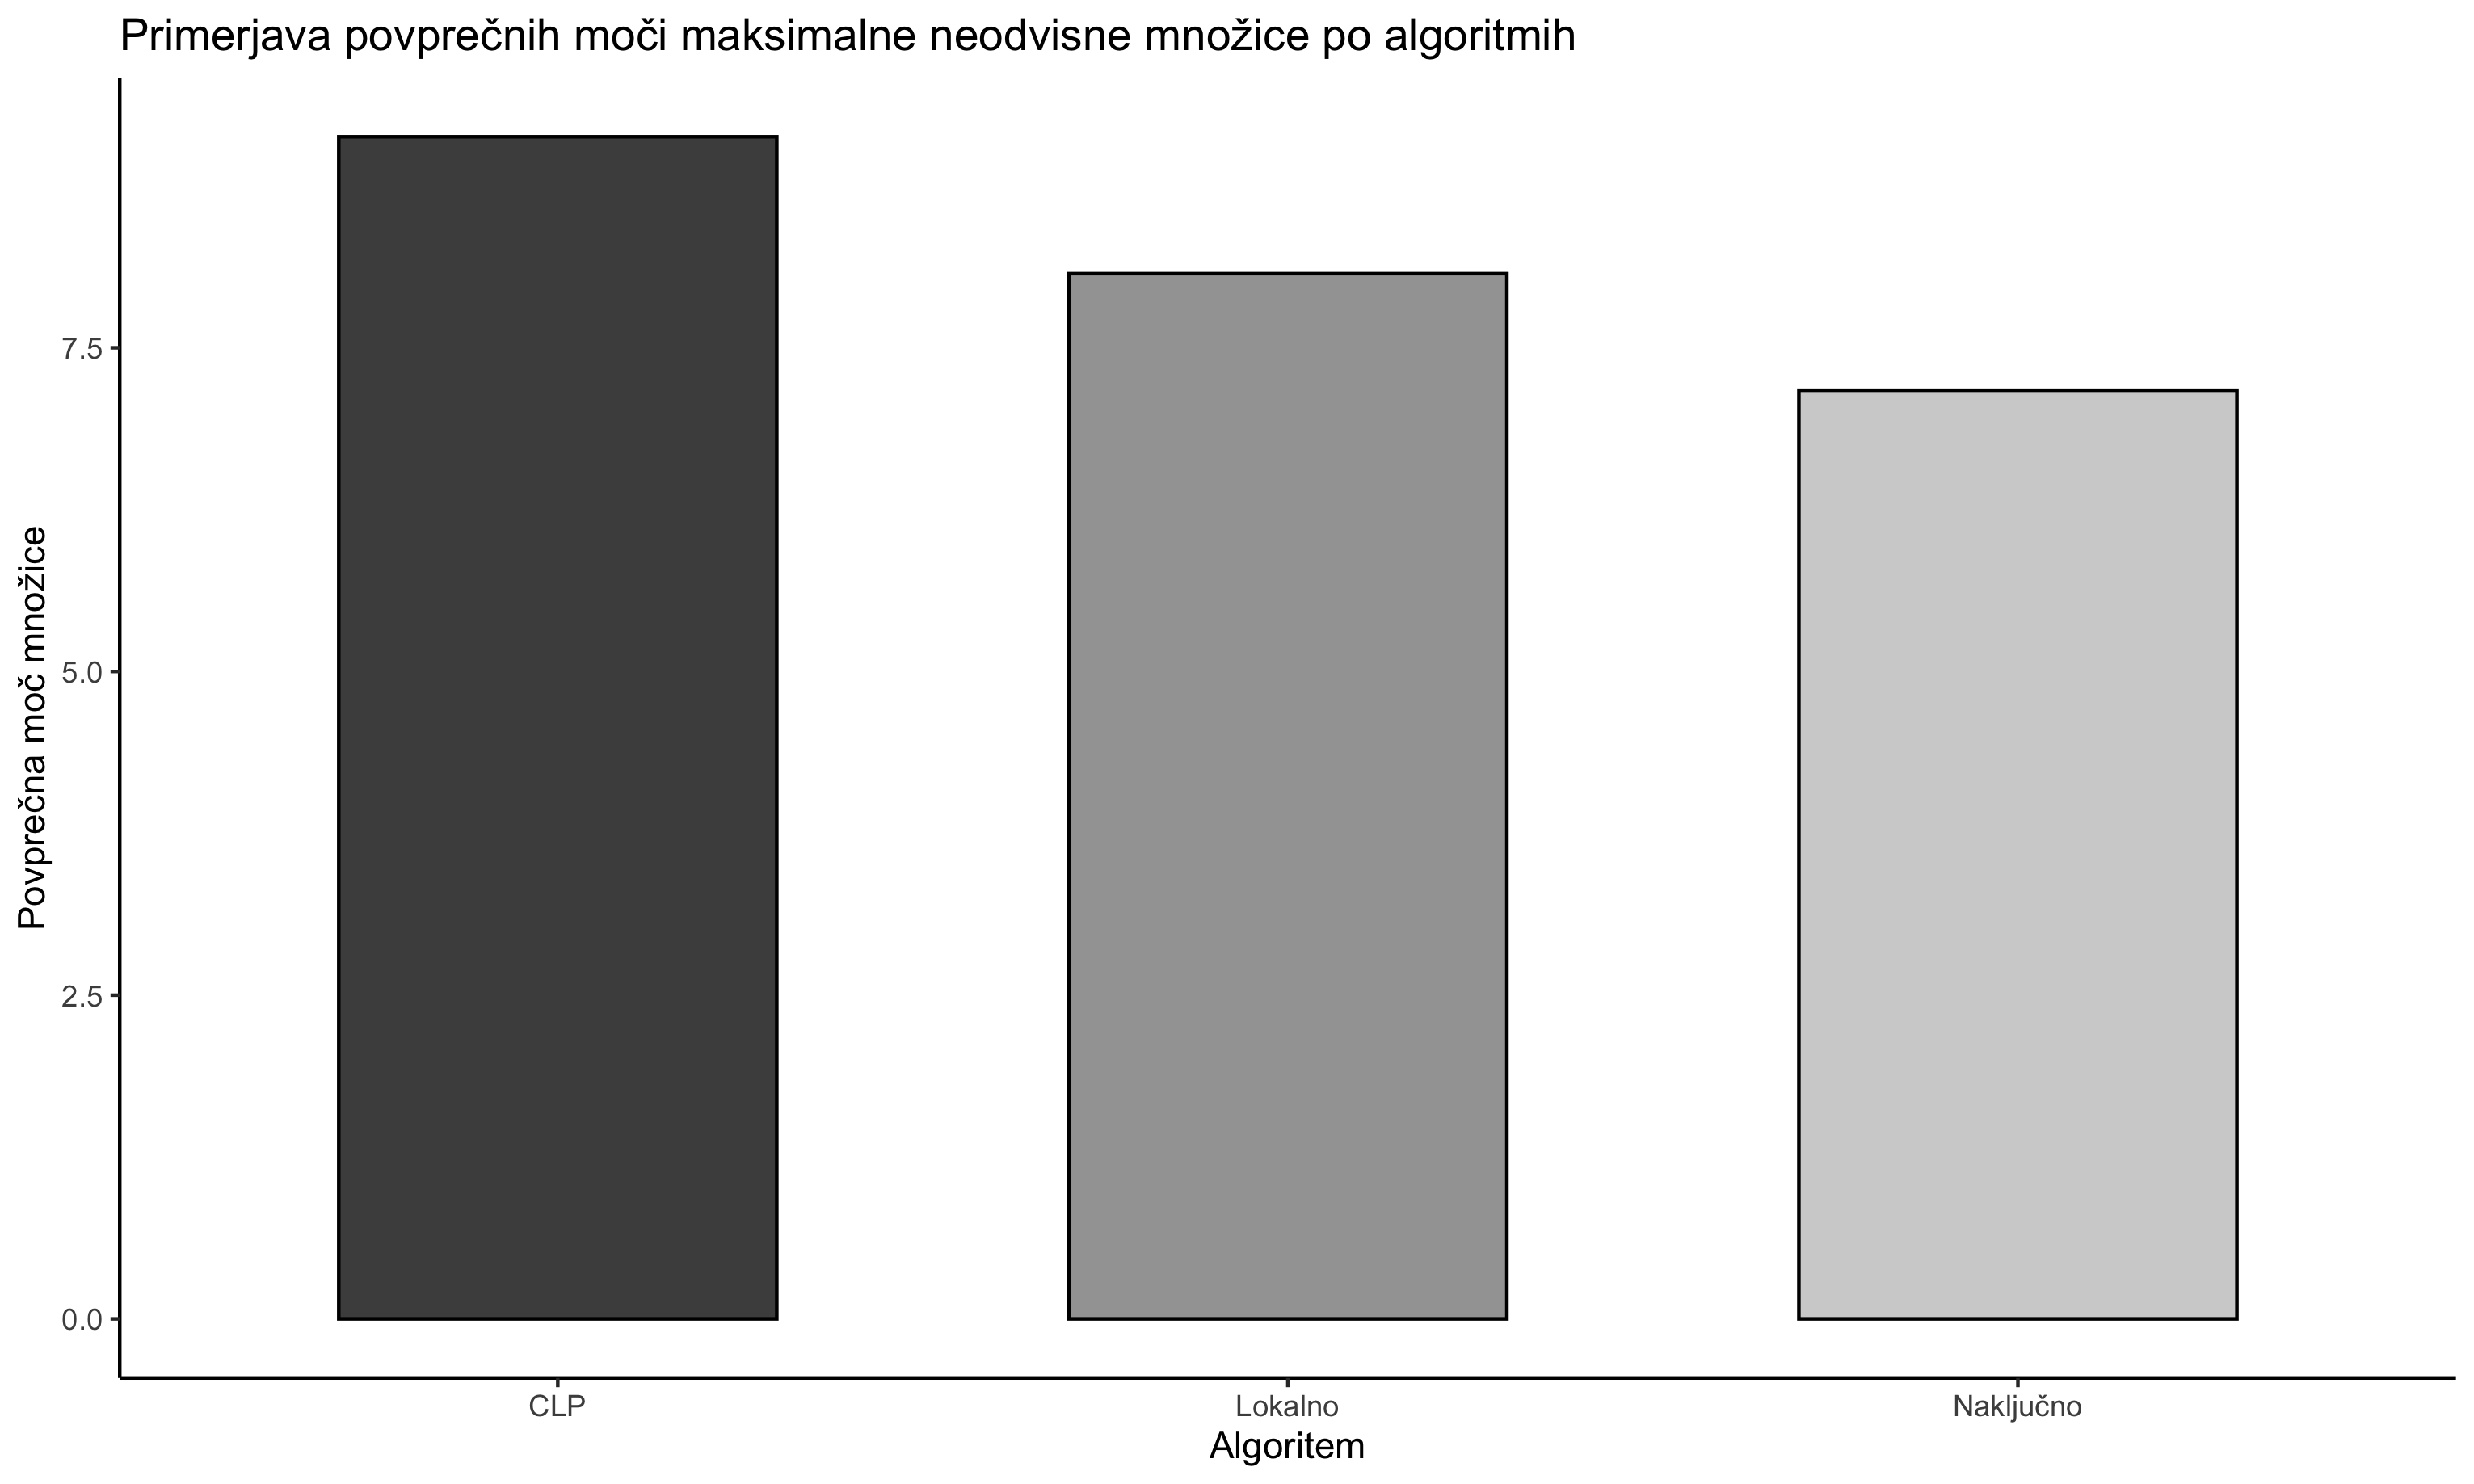
\includegraphics[scale=0.11]{R_koda/pon-povpmoc.png}
		\caption{Povprečne vrednosti rezultatov posameznih algoritmov}
	\end{center}
\end{figure}

\subsubsection{Analiza izboljšanih algoritmov na grafih $G(50, 0.3)$}

\noindent V nadaljevanju sva poskusila rezultat dobljen z $lokalnim\_iskanjem$ in algoritmom \textit{nakljucni\_MIS} nekoliko izboljšati. 
Najprej sva za rešitev dobljeno z $nakljucni\_MIS$ vzela najboljšo izmed dvajsetih simulacij za vsak graf, kar je na spodnjem grafu označeno z 
\textit{Naključno najboljša}. Iz te dobljene neodvisne množice sva potem izhajala pri $lokalnem\_iskanju$ in rešitev označila kot
\textit{Lokalno najboljša}. Rešitev dobljena s $CLP$ je še zmeraj enaka, sva pa dobila še maksimalne neodvisne množice na način, da sva algoritem $lokalno\_iskanje$
pognala na 10 različnih začetnih neodvisnih množicah, dobljenih z $nakljucni\_MIS$. Na grafu je ta rešitev označena z \textit{Lokalno različne neodvisne množice} in kot je razvidno, 
sva na ta način dobila najboljše rezultate. V tem primeru celo boljše od $CLP$.

\begin{figure}[h!]
	\begin{center}
		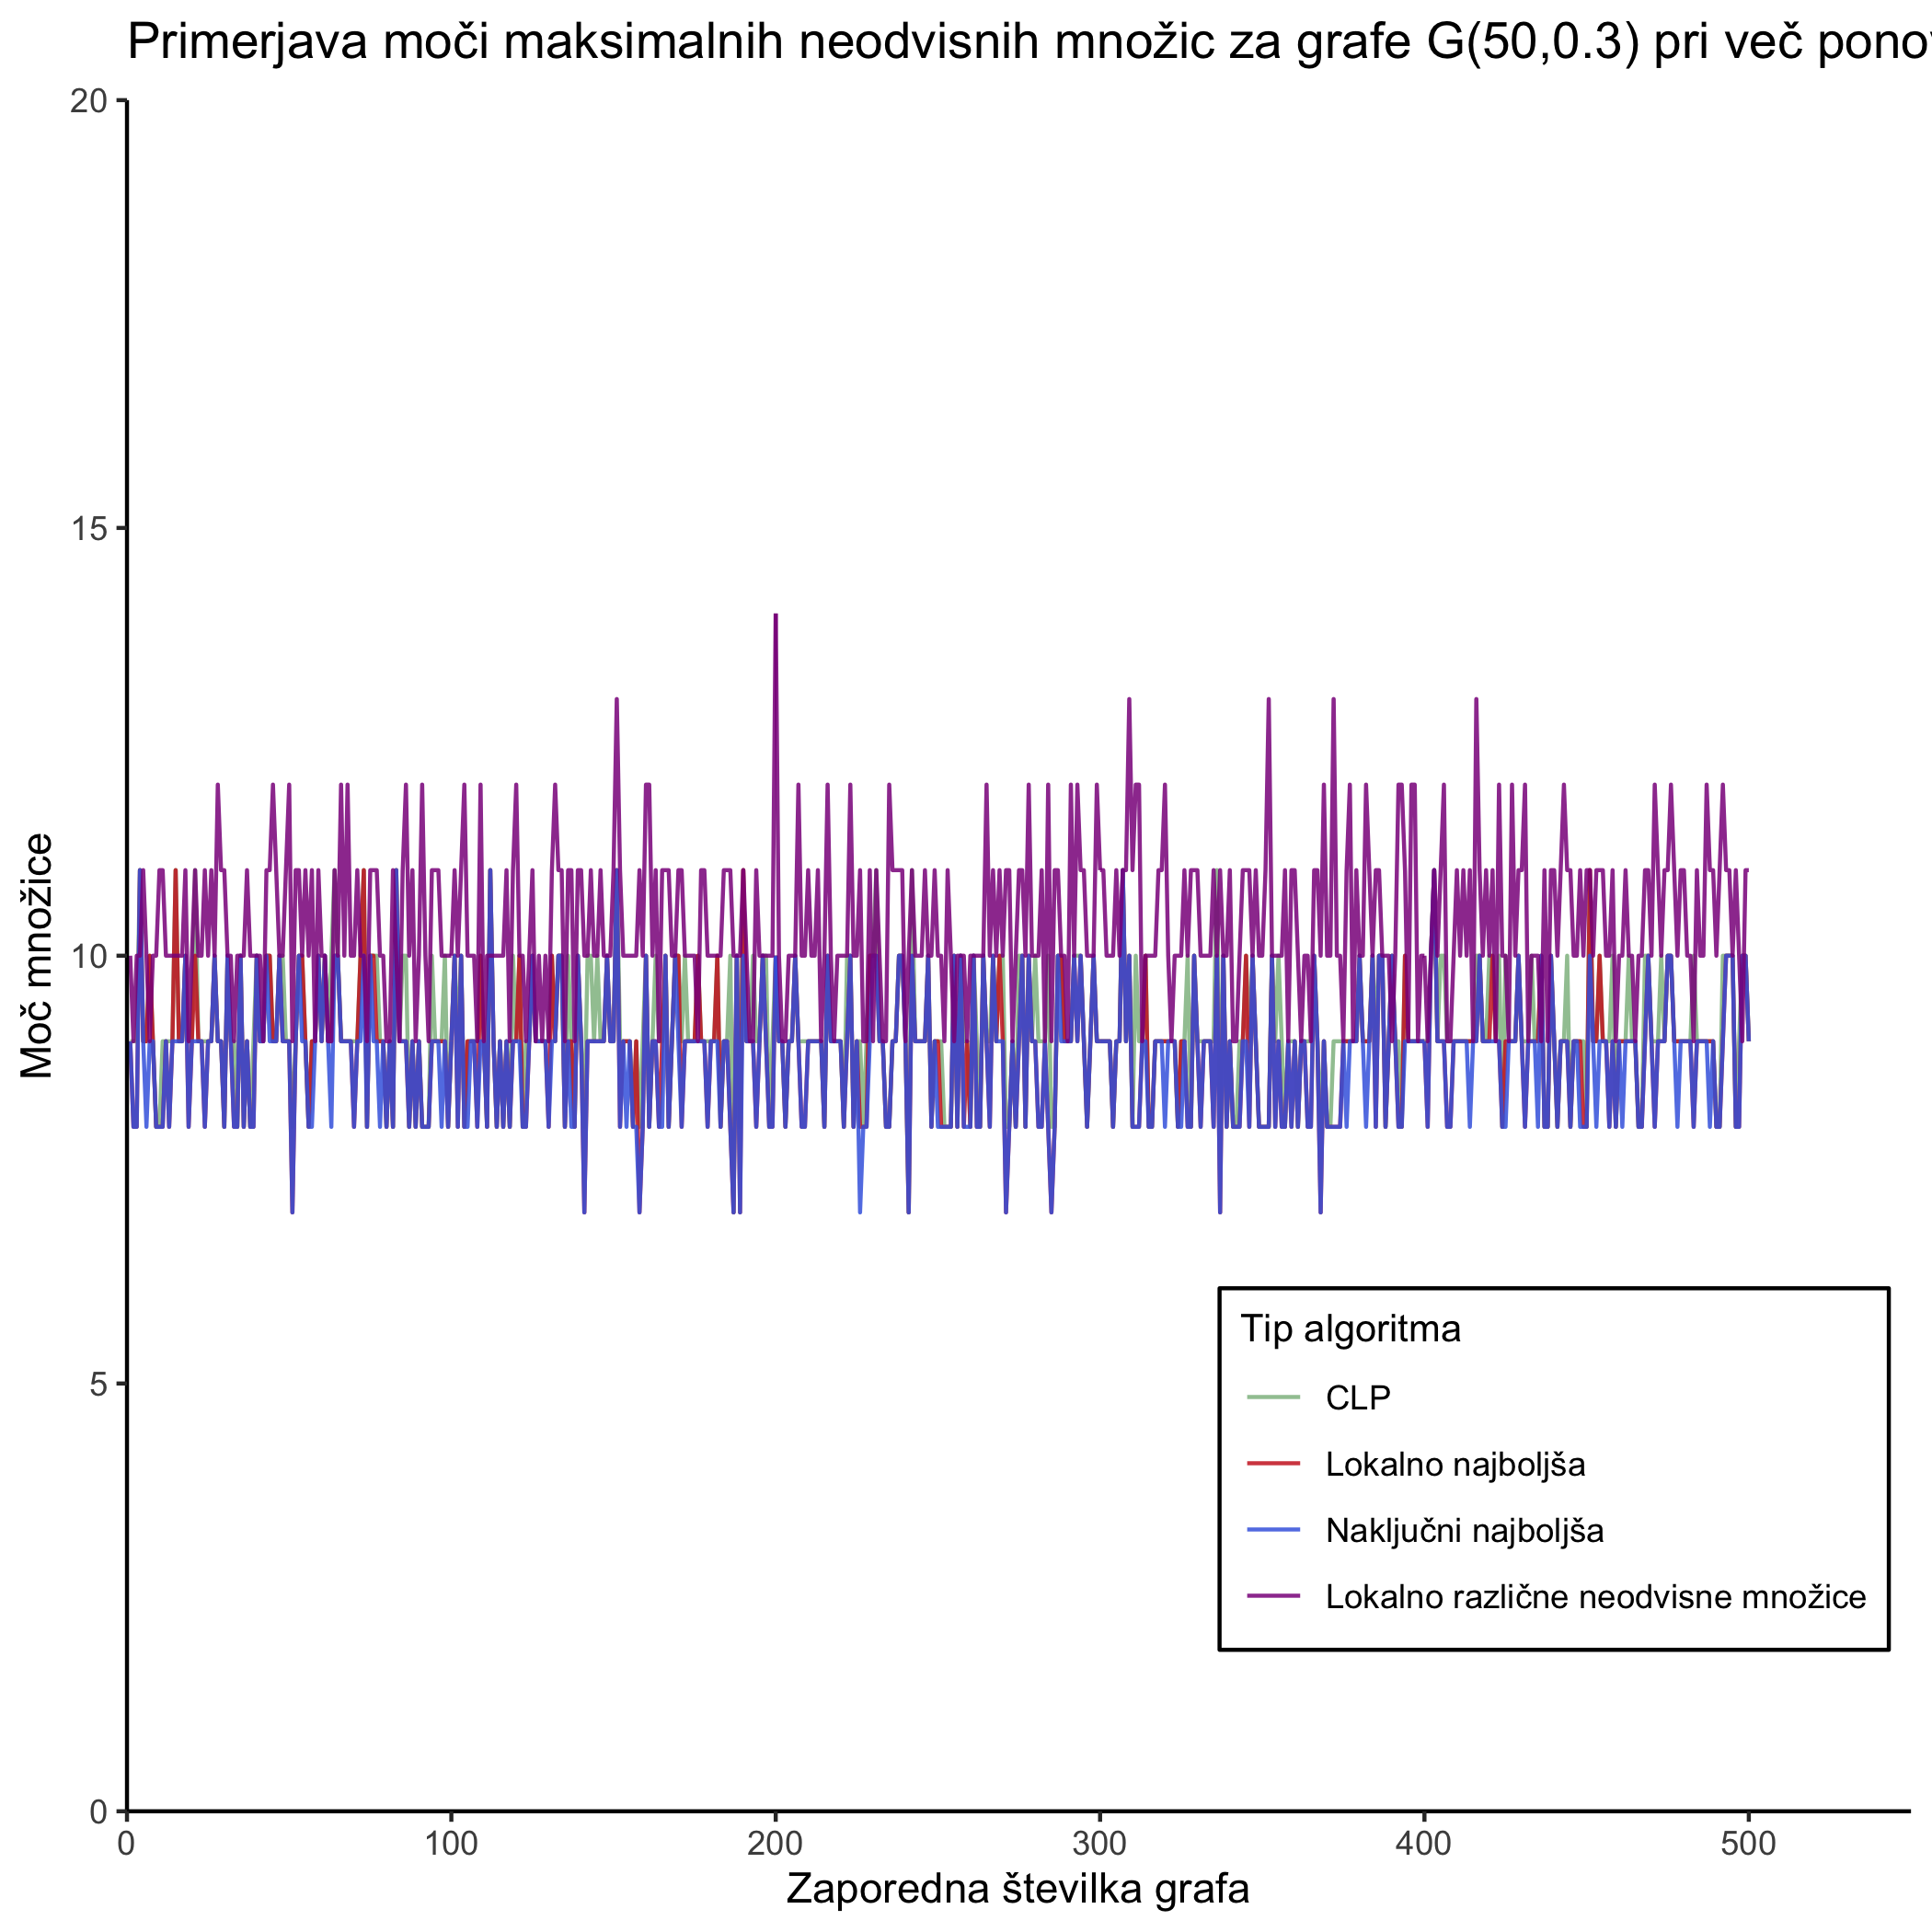
\includegraphics[scale = 0.11]{R_koda/pon-moc-maximalno.png}
		\caption{Vrednosti rezultatov izboljšanih posameznih algoritmov}
	\end{center}
\end{figure}

\noindent Za zgoraj opisane postopke sva nato izmerila še čase izvajanja. Zelo zanimivo je dejstvo, da najboljše rešitve dobimo s časovno najbolj učinkovitim algoritmom.
Vmes se pojavijo tudi kakšni izraziti skoki, ki pa jih lahko pripišemo slučaju, saj je čas izvajanja zelo odvisen od vrste grafa, na katerem se algoritem izvede.
Ker grafe generirava naključno je prav to vzrok za opažene osamelce.

\begin{figure}[h!]
	\begin{center}
		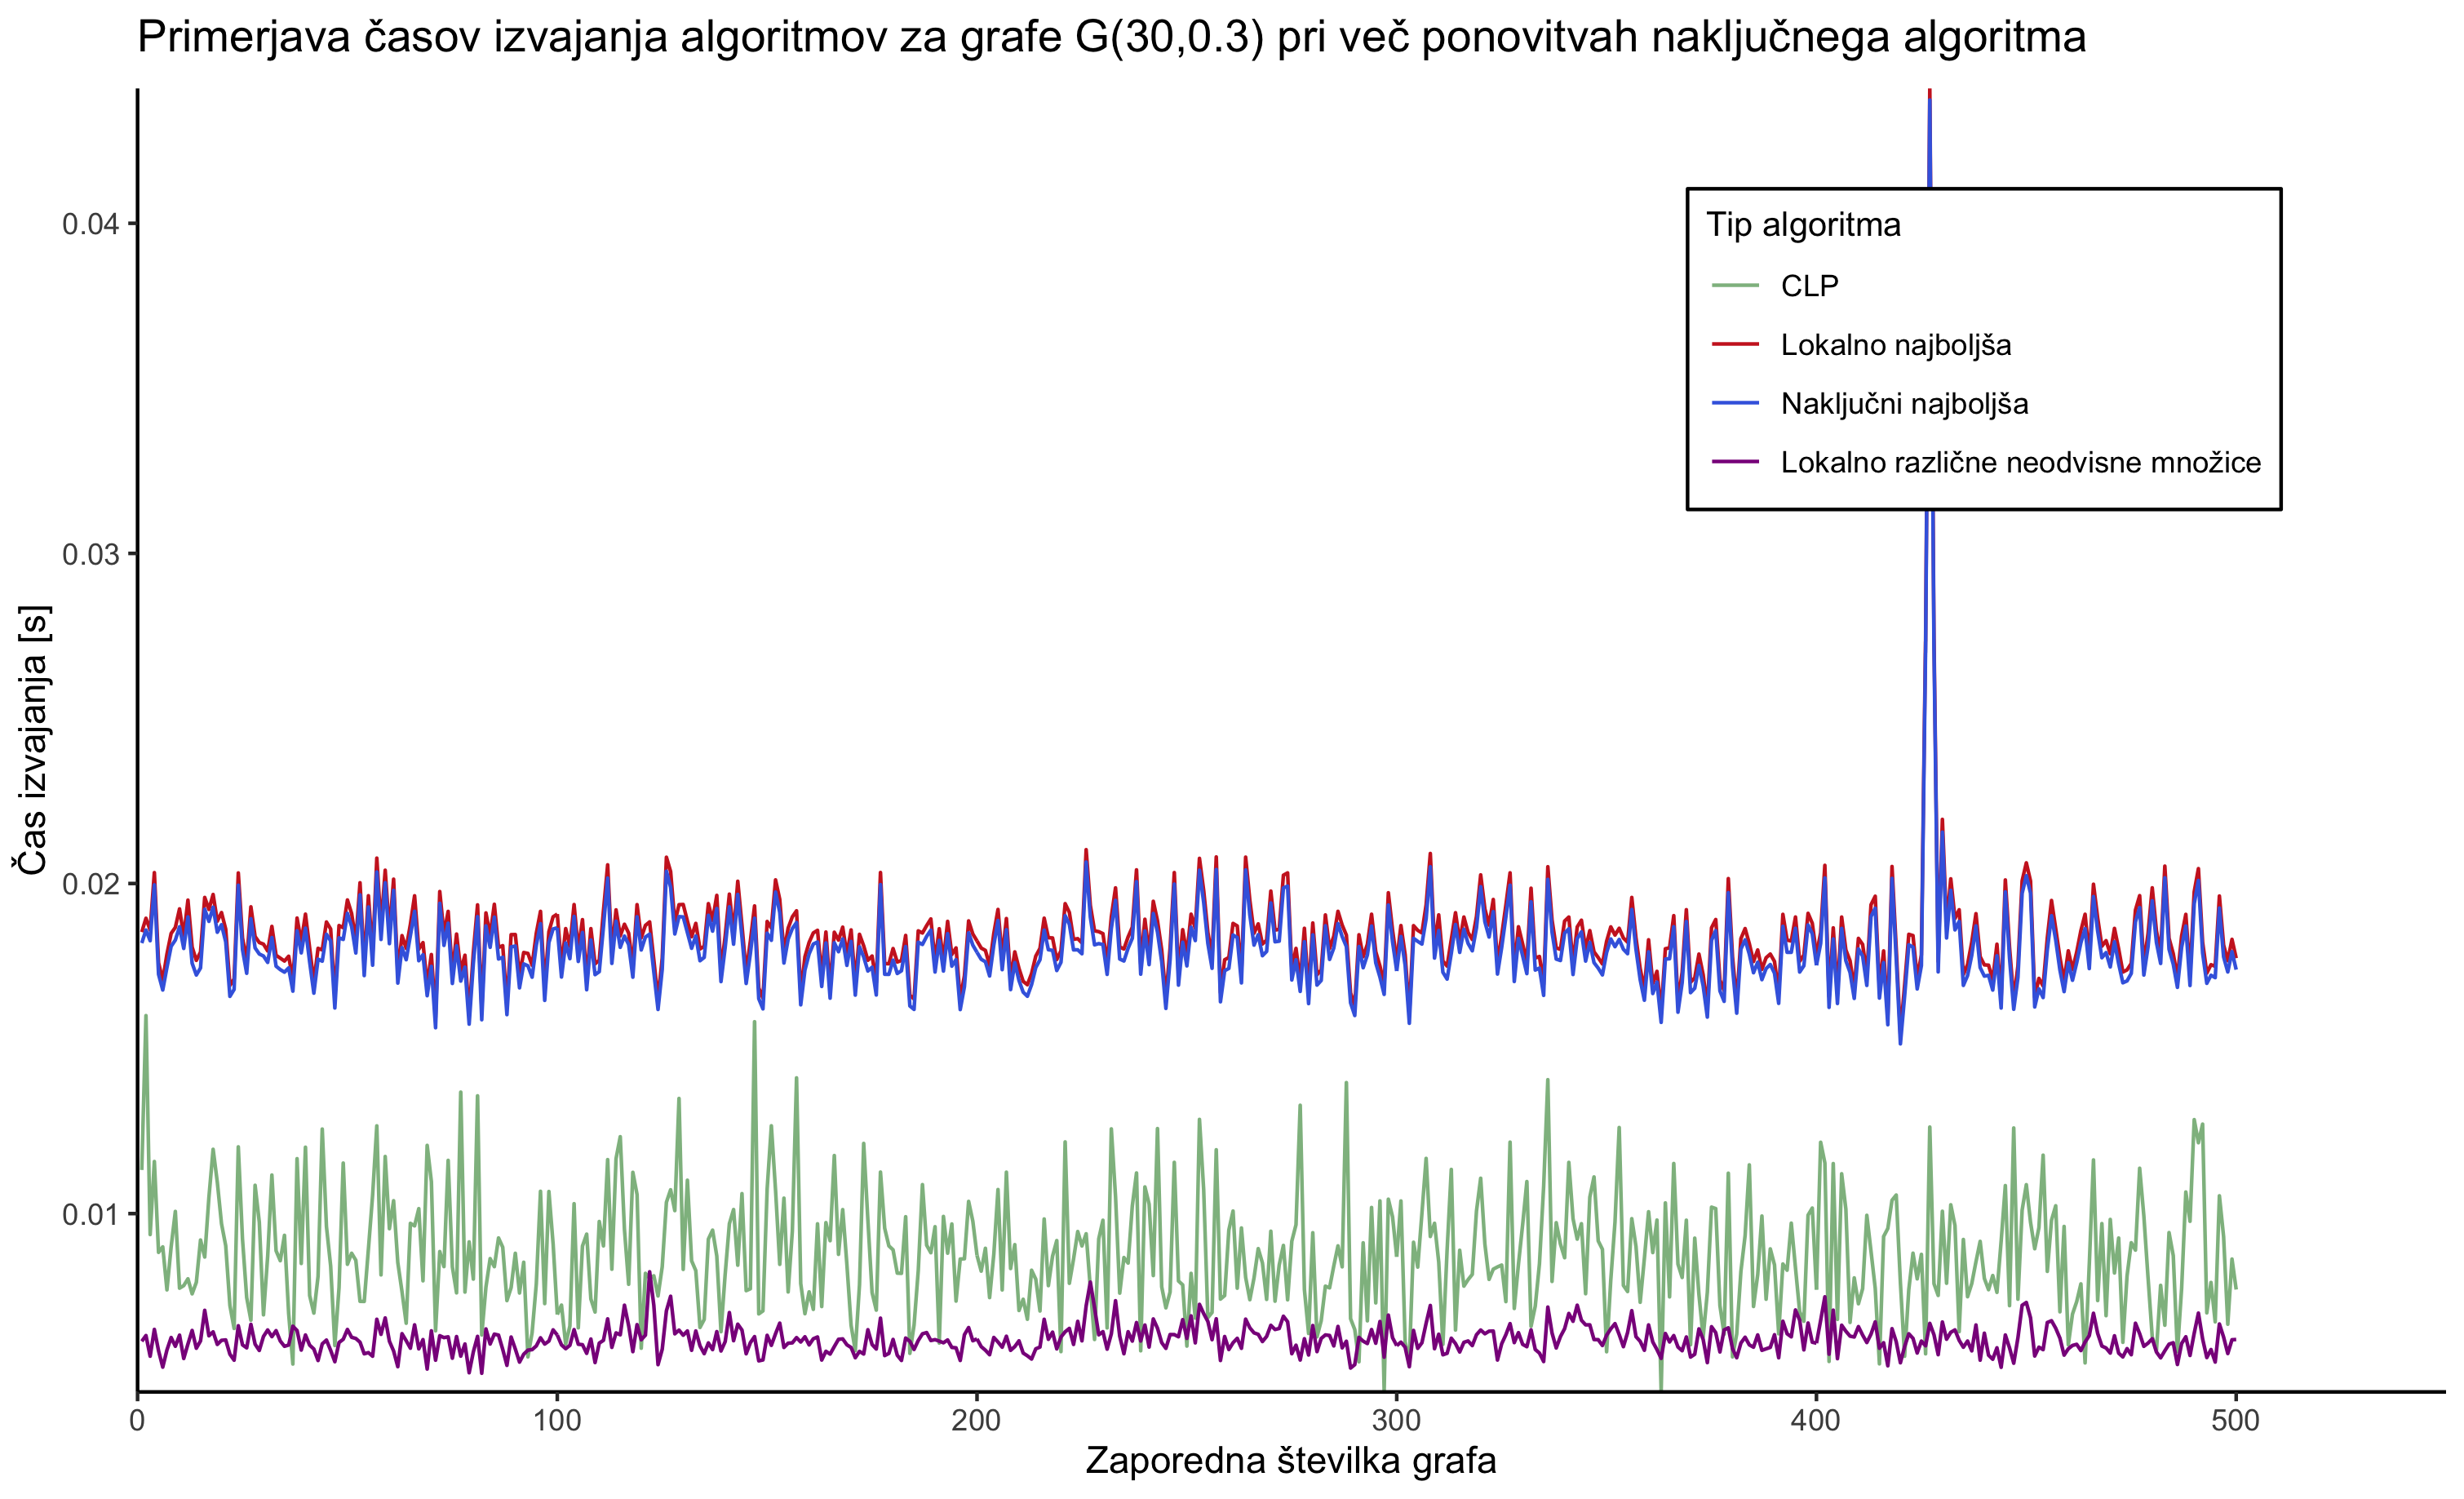
\includegraphics[scale=0.11]{R_koda/pon-casi-maxi.png}
		\caption{Časovne zahtevnosti izboljšanih posameznih algoritmov}
	\end{center}
\end{figure}


\noindent Da bi se res transparentno prepričali, da v tem primeru najboljše rešitve v povprečju poiščeva z \textit{Lokalno različne neodvisne množice}, ko naredimo algoritem $lokalno\_iskanje$
na različnih začetnih neodvisnih množicah, sva izračunala povprečne moči, ki jih vračajo algoritmi. Na spodnjem grafu lahko to očitno opazimo.
\begin{figure}[h!]
	\begin{center}
		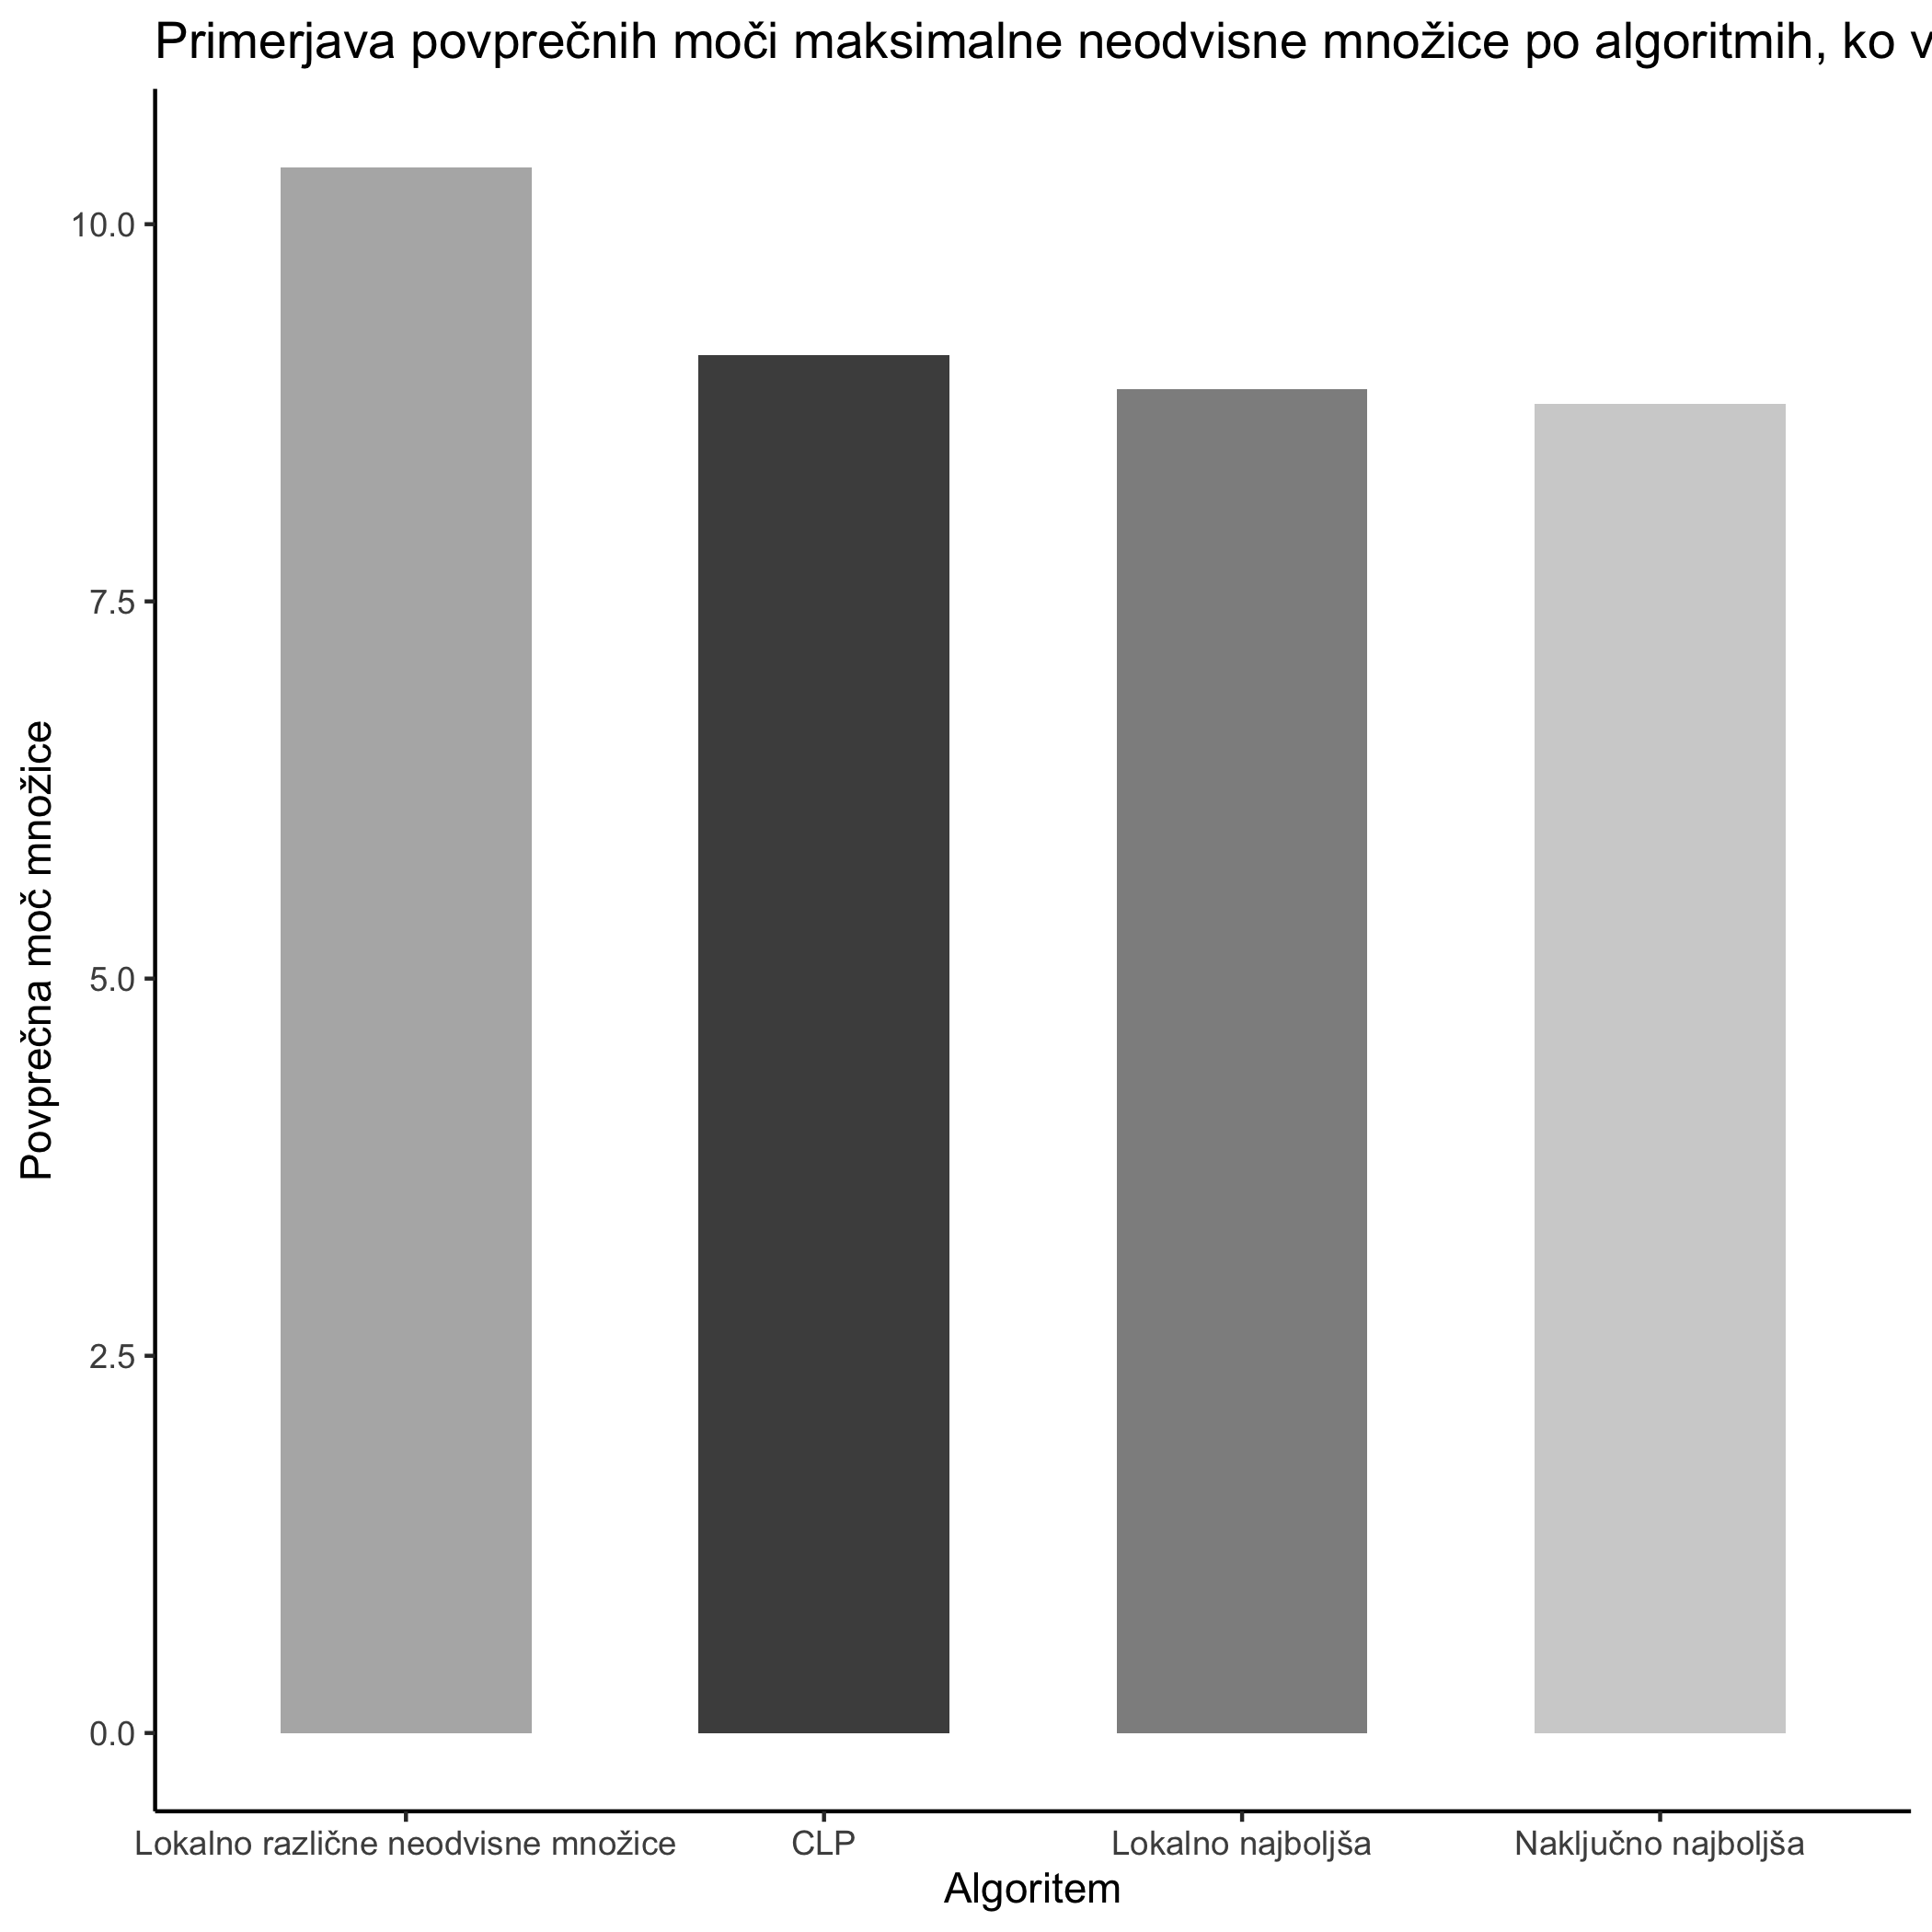
\includegraphics[scale=0.12]{R_koda/pon-povpmoc-maxi.png}
		\caption{Povprečne vrednosti rezultatov izboljšanih posameznih algoritmov}
	\end{center}
\end{figure}

\subsubsection{Primerjava algoritmov na grafih s konstantno verjetnostjo $p$ in spremenljivim številom vozlišč $n$}

Drugo skupino grafov sva, tako kot prvo, generirala z $\text{Erdős-Rényijevim}\ G(n, p)$ modelom, vendar pri tem spreminjala število vozlišč v grafih, verjetnost pa ohranila konstantno $p=0.005$.
Algoritme sva izvajala na grafih velikosti od 1 do 600 vozlišč. Ker je verjetnost konstantna, na rezultate ne vpliva in tako sva si lahko izbrala grafe na večjem številu vozlišč ter pridobila več podatkov za bolj natančno analizo rezultatov.\\

\noindent Na spodnjem grafu si lahko ogledamo kako se s povečevanjem števila vozlišč, spreminja moč maksimalnih neodvisnih množic. Pri konstantni verjetnosti $p$, se moč maksimalne neodvisne množice, v odvisnosti od 
moči množice vozlišč $V$, povečuje skoraj linearno, vendar moč maksimalnih neodvisnih množic dobljenih s $CLP$ narašča hitreje od tistih pridobljenih z $nakljucni\_MIS$ in
$lokalnim\ iskanjem$.

\newpage

\begin{figure}[h!]
	\begin{center}
		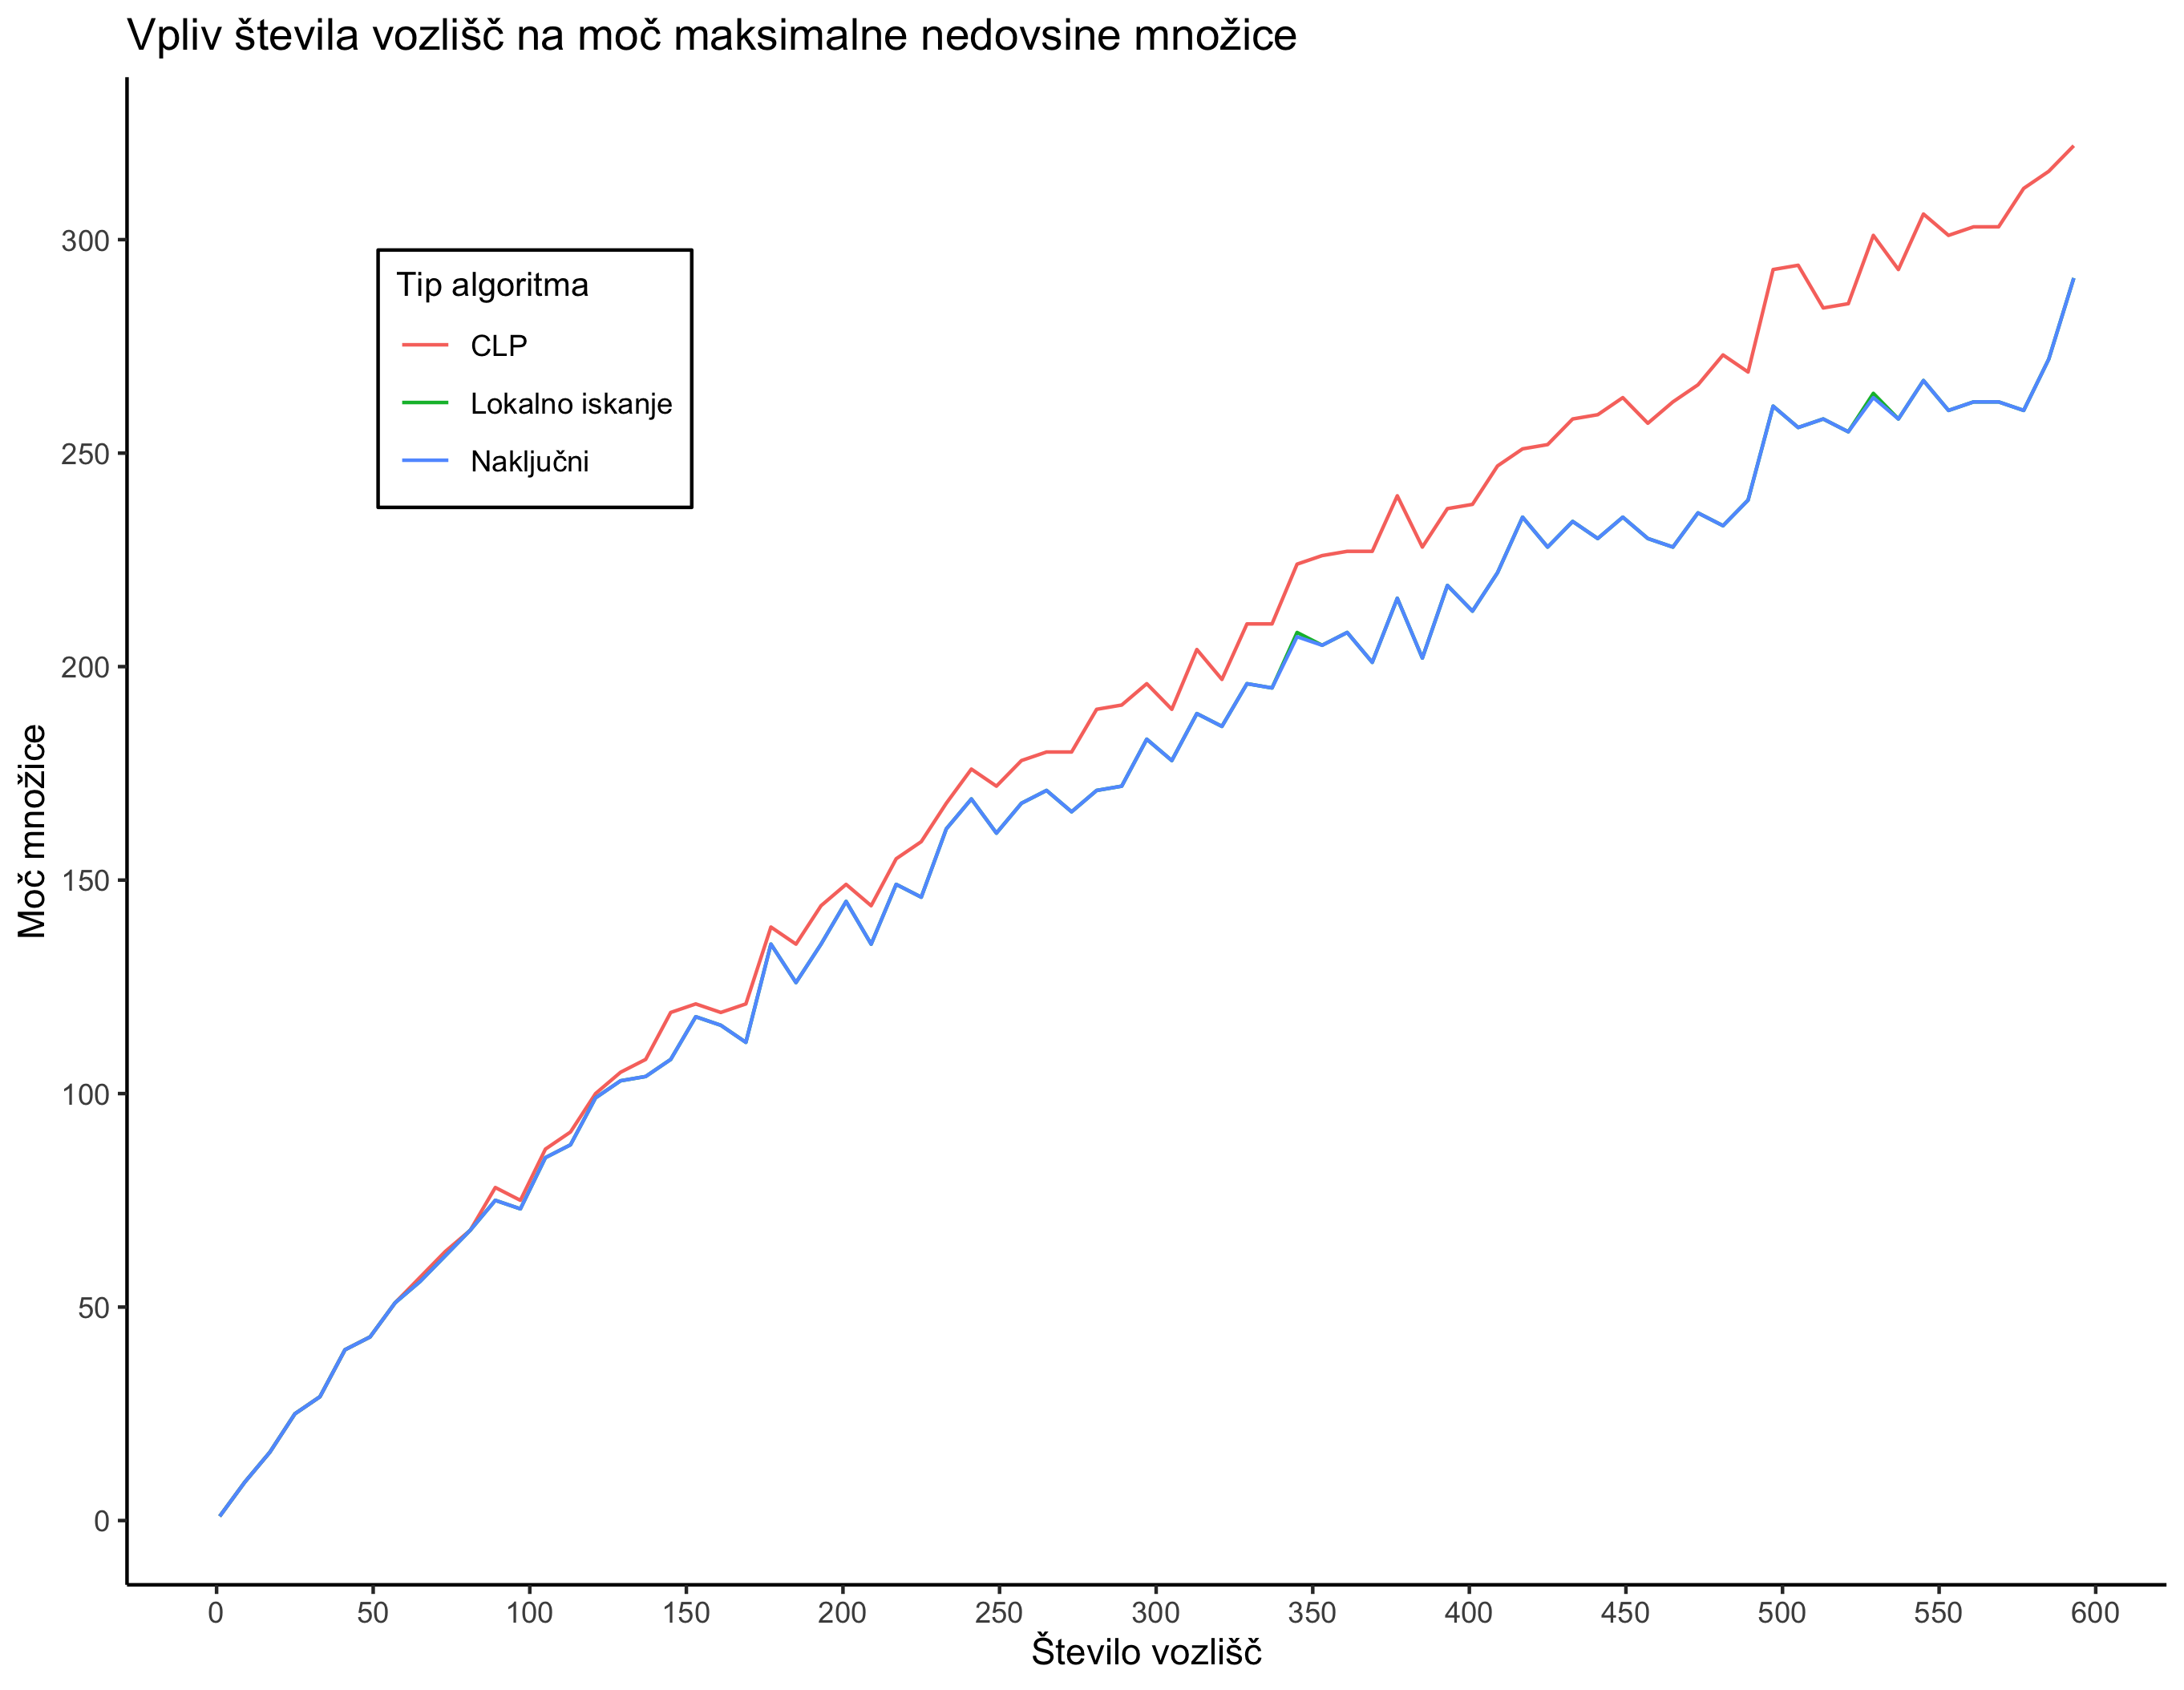
\includegraphics[scale=0.11]{R_koda/voz-moc.png}
		\caption{Velikosti neodvisnih množic v odvisnosti od števila vozlišč $n$}
	\end{center}
\end{figure}

\noindent Na spodnjem grafu ponovno opazimo največjo slabost iskanja maksimalne neodvisne množice s $CLP$, tj. časovno zahtevnost. Čas, porabljen za izvajanje $CLP$, je v odvisnosti od števila vozlišč v množici $V$
naraščal eksponentno. Prav tako je naraščala časovna zahtevnost algortimov $nakljucni\_MIS$ in $lokalnega\_iskanja$, vendar so bila naraščanja na opazovanih grafih občutno manjša.
Glede na to, da je iskanje maksimalne neodvisne množice $NP$-težek problem lahko pričakujemo, da bi z nadaljnjim povečevanjem števila vozlišč v množici $V$ časovna zahtevnost začela naraščati
eksponentno tudi za druga dva algoritma. Zametki tega so opazni, ko gledamo časovne zahtevnosti algoritmov $nakljucni\_MIS$ in $lokalnega\ iskanja$ za največje moči množice $V$, na skrajnem desnem robu grafa.


\begin{figure}[h!]
	\begin{center}
		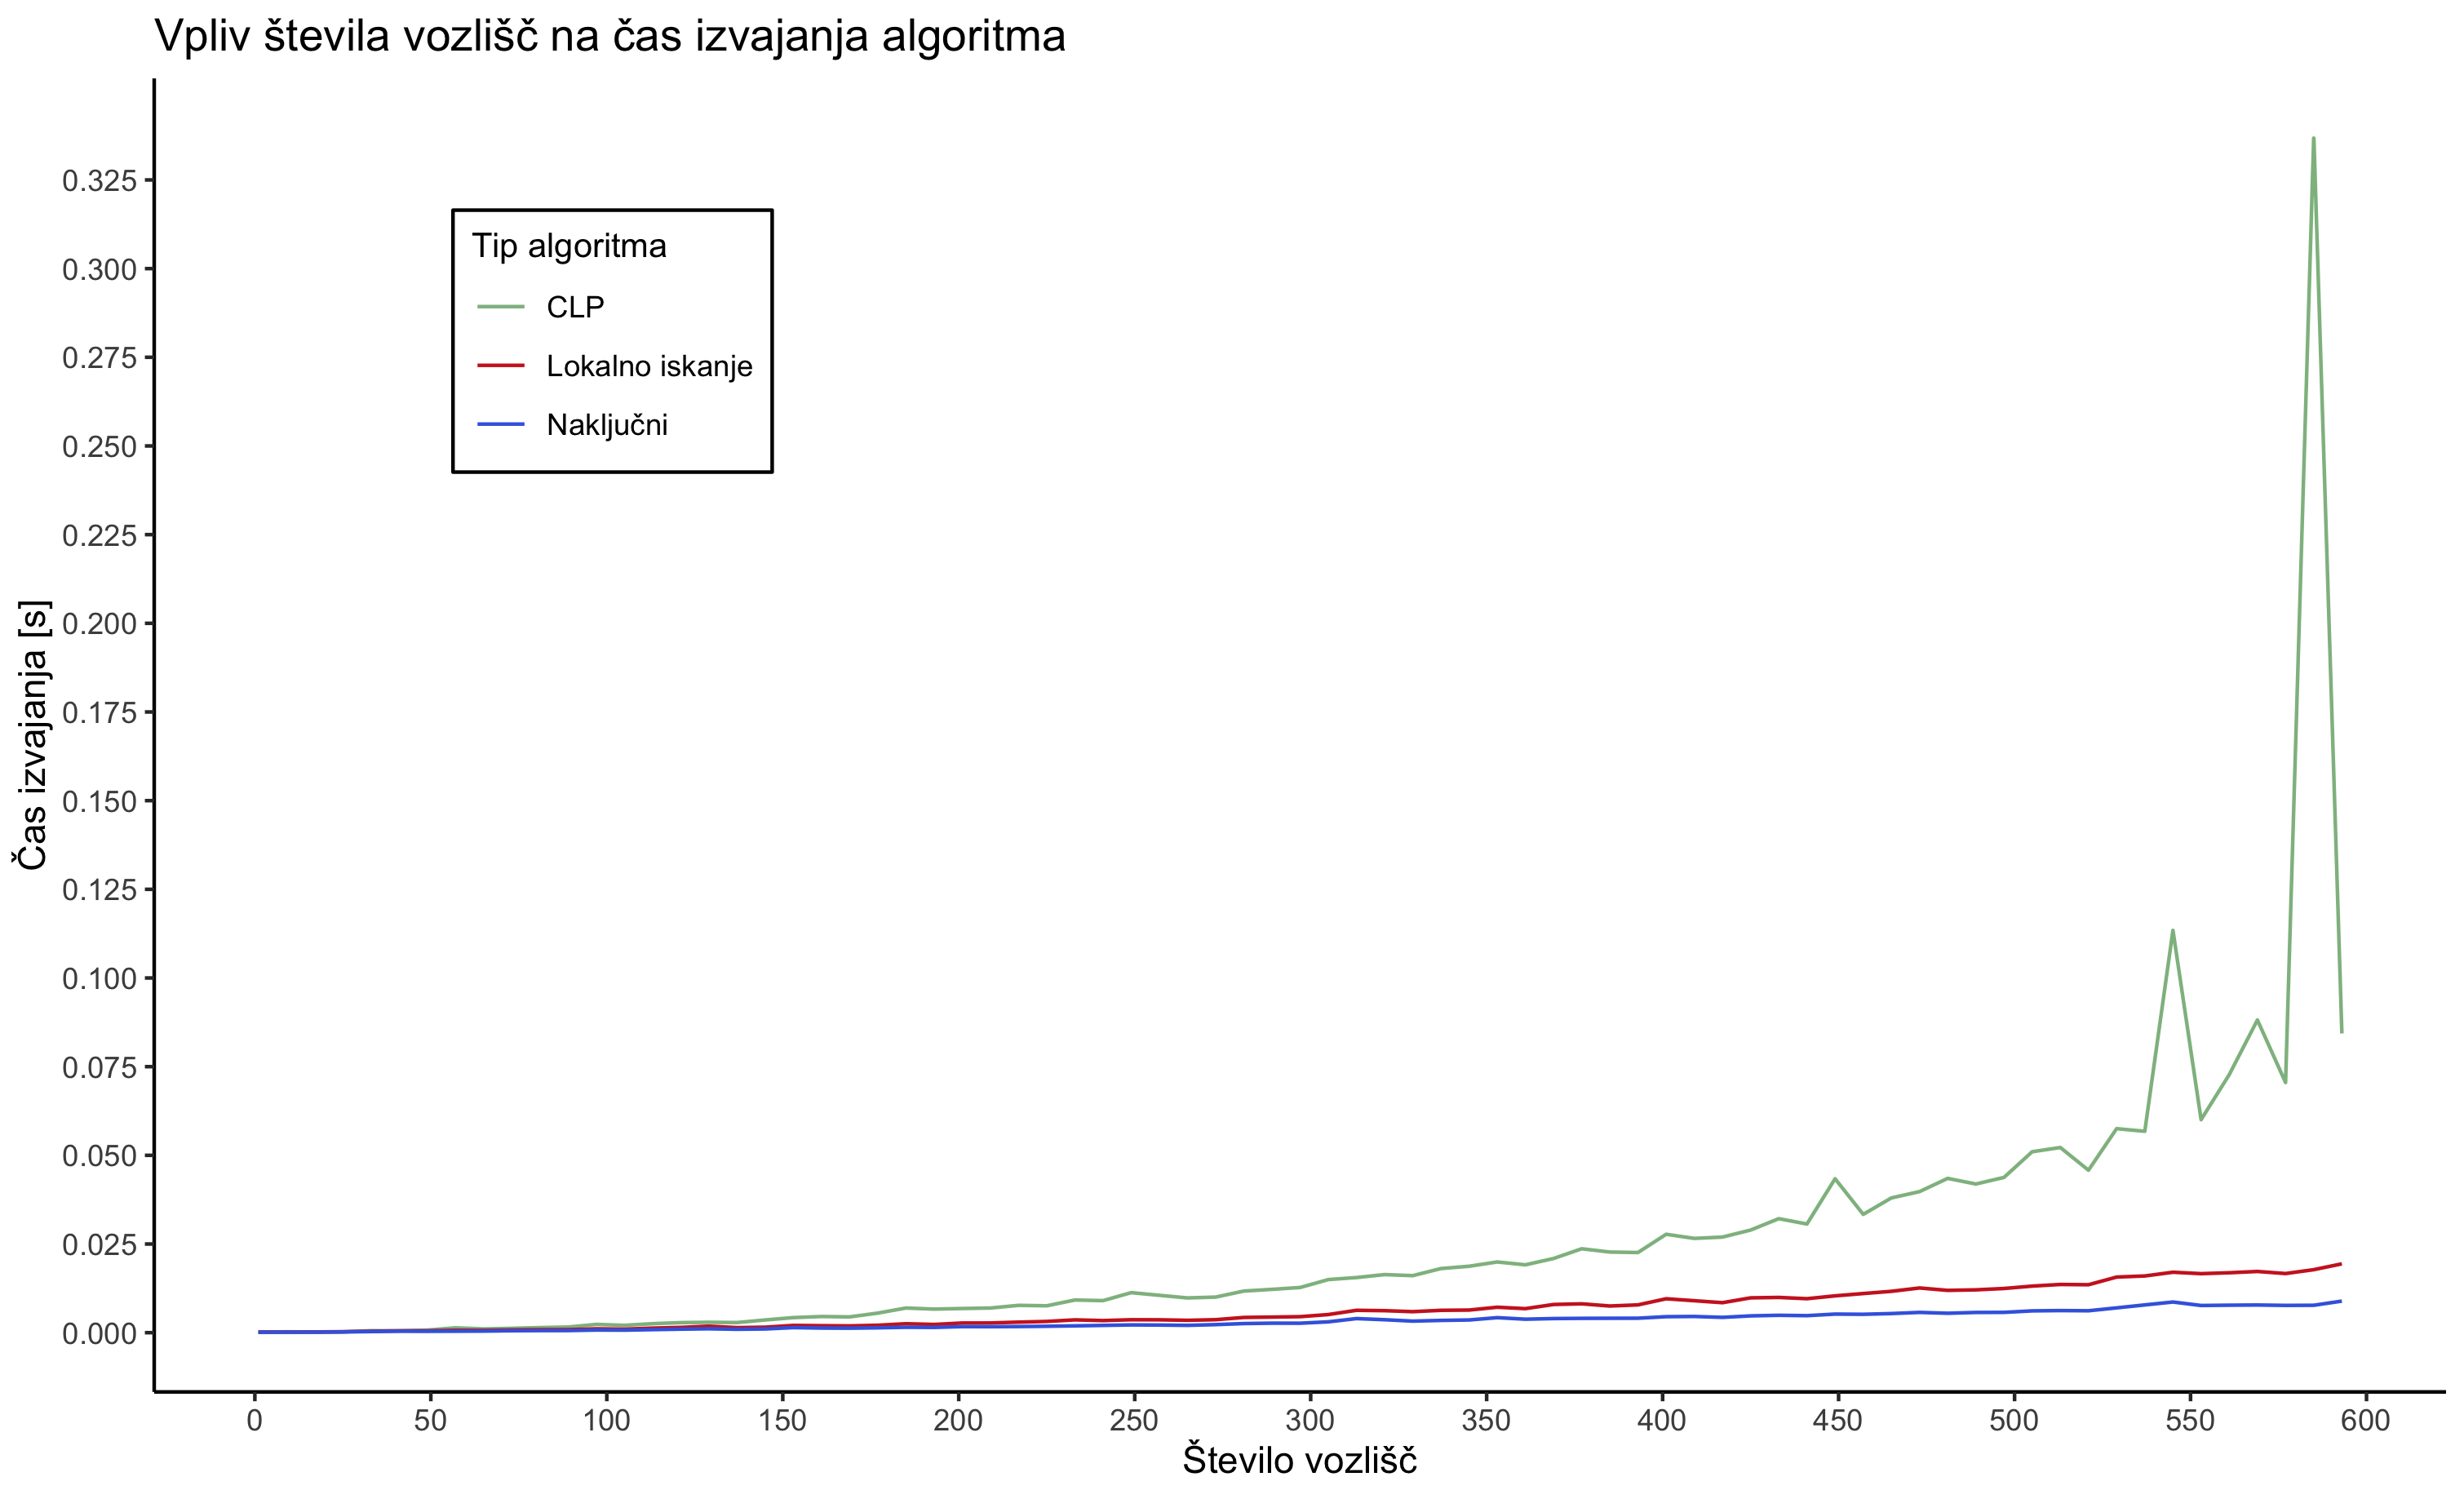
\includegraphics[scale=0.11]{R_koda/voz-cas.png}
		\caption{Spreminjanje časovne zahtevnosti algoritmov v odvisnosti od števila vozlišč $n$}
	\end{center}
\end{figure}


\subsubsection{Primerjava algoritmov na grafih s konstantim številom vozlišč $n$ in s spremenljivo verjetnostjo $p$}

Tudi zadnjo skupino grafov sva generirala z $\text{Erdős-Rényijevim}\ G(n, p)$ modelom, pri tem pa ohranila konstantno velikost množice vozlišč $V$ in spreminjala verjetnosti $p$.
Vrednosti verjetnosti sva dobila s klicom funkcije $numpy.linspace(0.1, 0.8, 80)$.\\

\noindent Če je s povečevanjem velikosti množice $V$ naraščala tudi velikost maksimalne neodvisne množice, opazimo, da je v primeru povečevanja verjetnosti $p$ vzorec nasproten, saj
velikost maksimalne neodvisne množice pada, ko povečujemo verjetnost $p$. Razlog za to se najvrjetneje skriva v vplivu verjetnosti na povezave grafa $G$. 
Večja kot je verjetnost $p$, večje bo število povezav v grafu, kar je za velikost neodvisne množice slabo, kar sledi neposredno iz definicije neodvisne množice. 
Torej velikost maksimalne neodvisne množice ni odvisna le od števila vozlišč v grafu, ampak tudi od števila povezav. Ugotovitve so opazne na spodnjem grafu.

\begin{figure}[h!]
	\begin{center}
		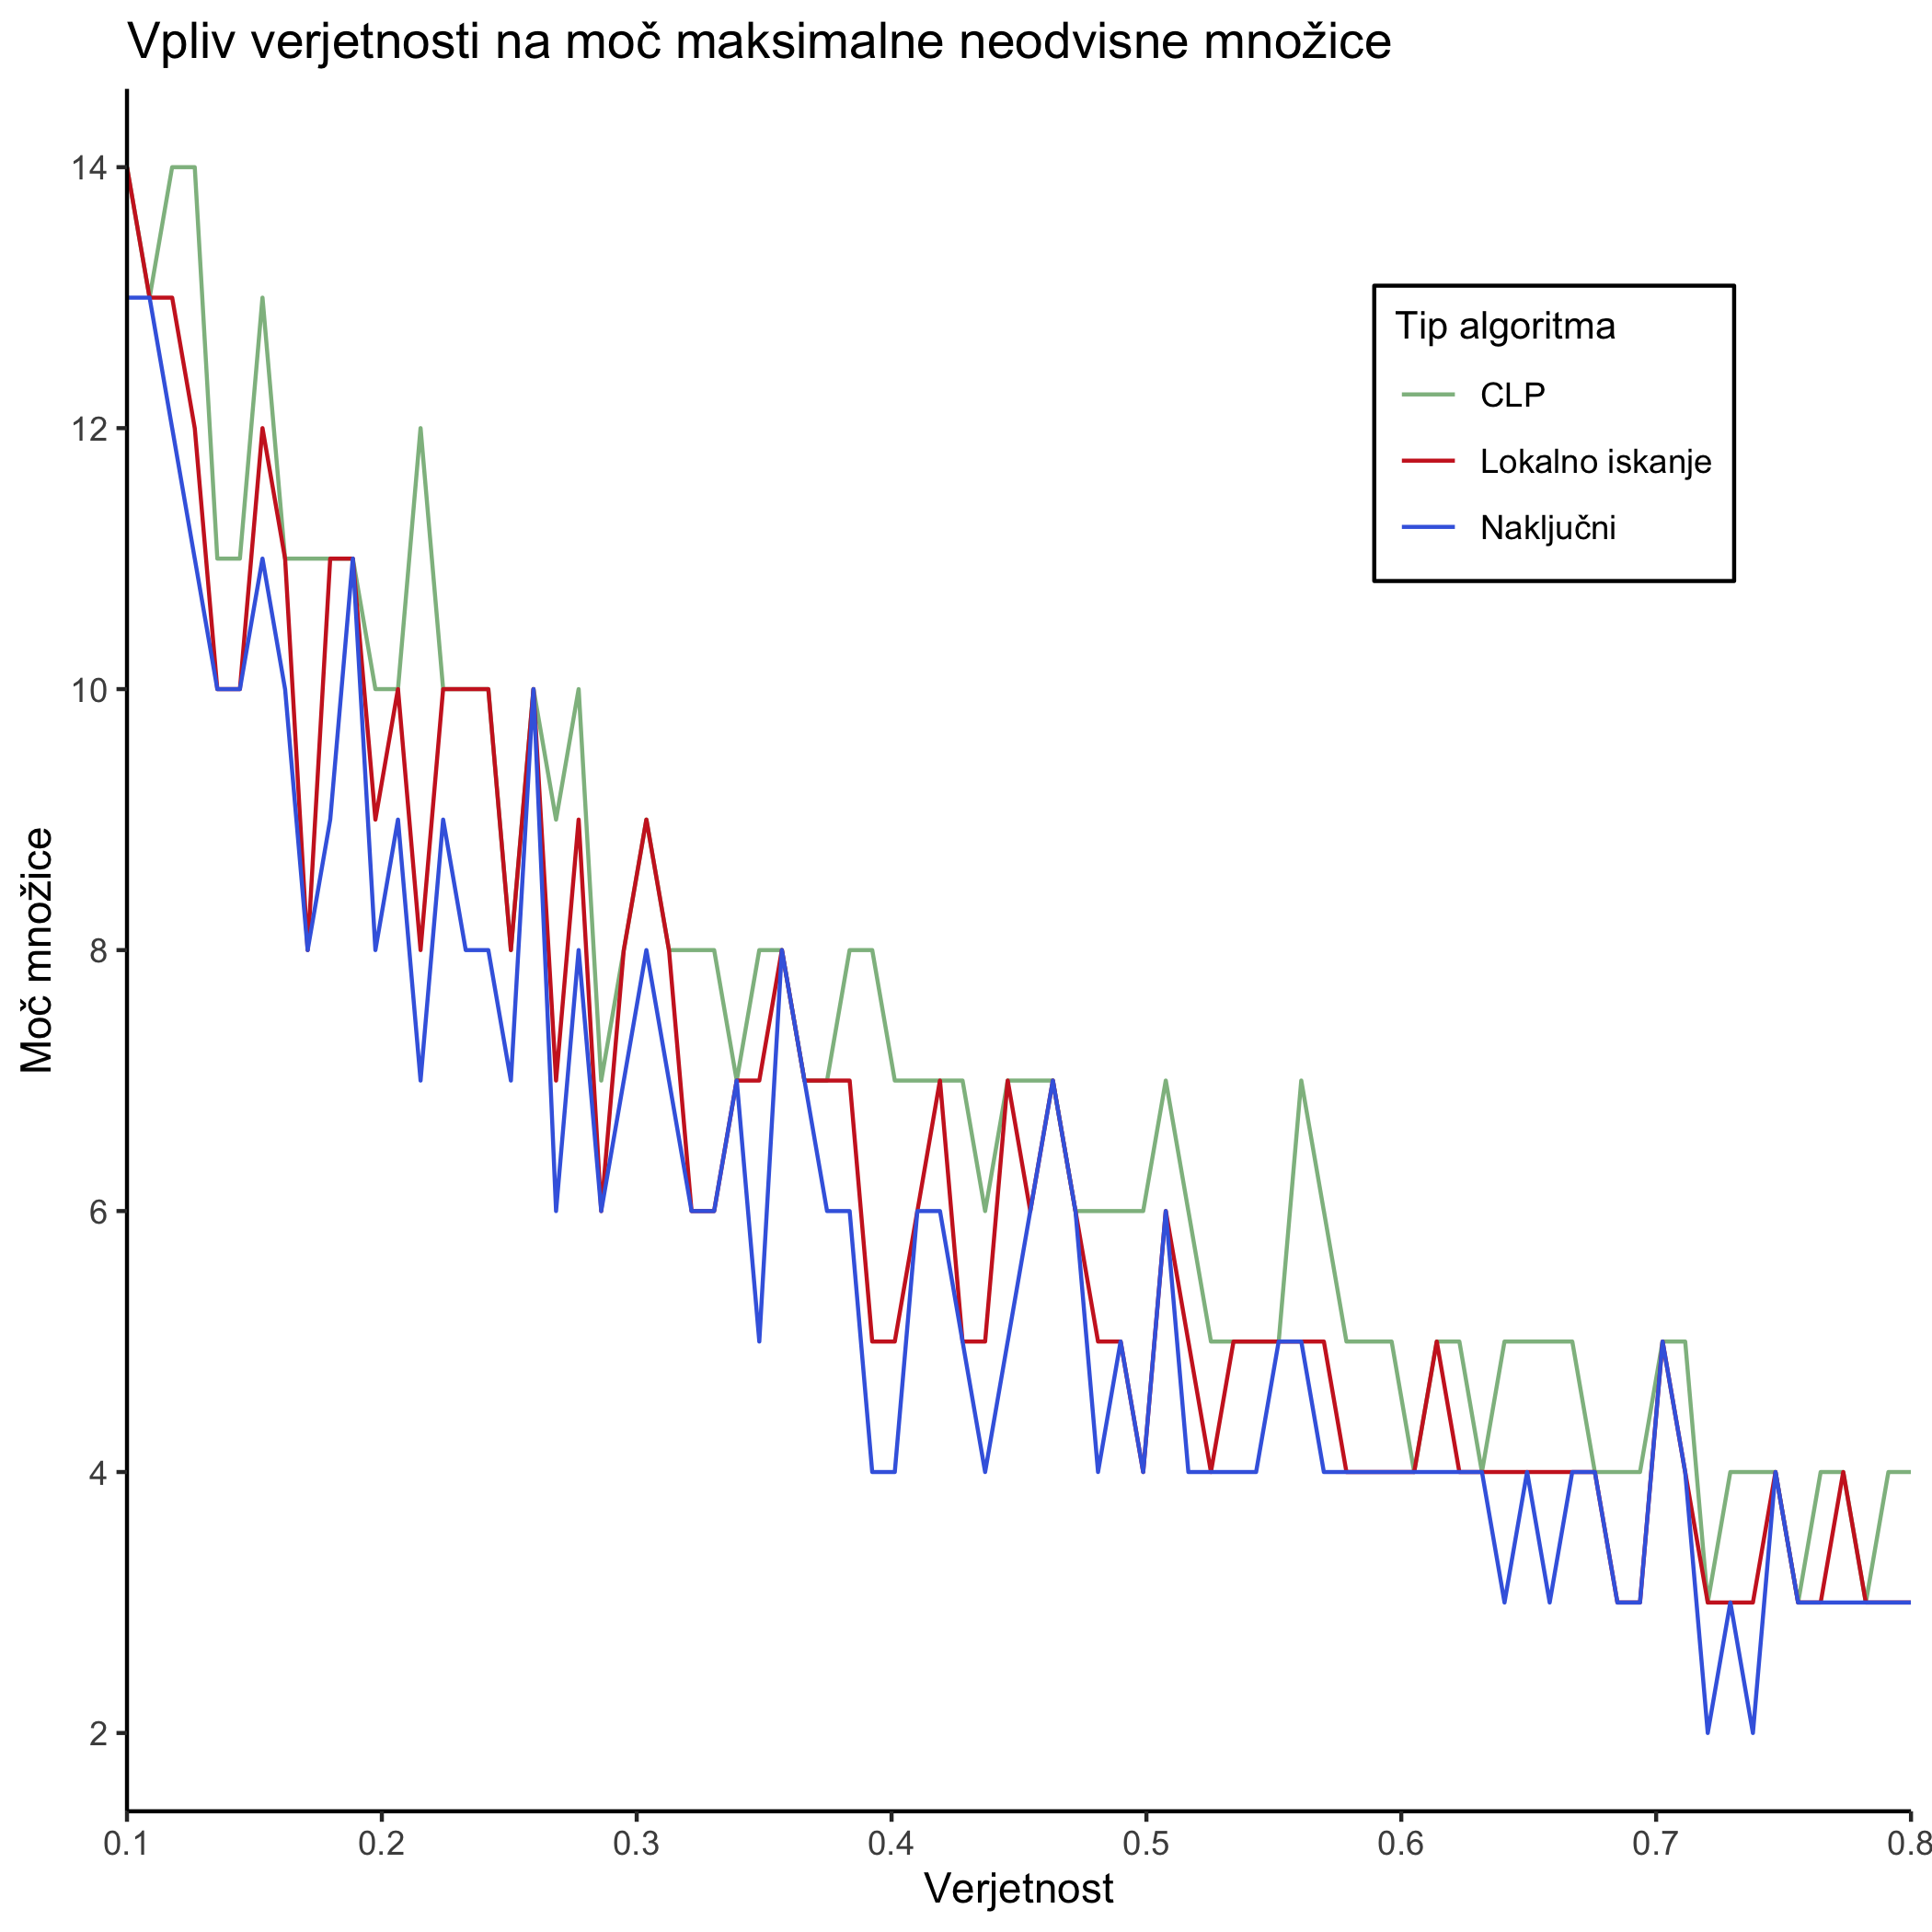
\includegraphics[scale=0.12]{R_koda/ver-moc.png}
		\caption{Vpliv verjetnosti na velikost neodvisnih množic}
	\end{center}
\end{figure}

\noindent Tako kot velikost maksimalne neodvisne množice, je od števila povezav v grafu (oz. verjetnosti $p$), odvisna tudi časovna zahtevnost algoritmov. Časovna zahtevnost algoritmov ob povečevanju verjetnosti $p$ 
(in posledično števila povezav v grafu) se obnaša podobno, kot se je obnašala pri povečevanju vozlišč. Časovna zahtevnost vseh treh algoritmov narašča z verjetnostjo $p$, vendar pri $CLP$ hitreje kot pri algoritmih
$nakljucni\_MIS$ in $lokalnim\ iskanjem$. Spodnji graf to nazorno prikazuje in potrjuje.

\begin{figure}[h!]
	\begin{center}
		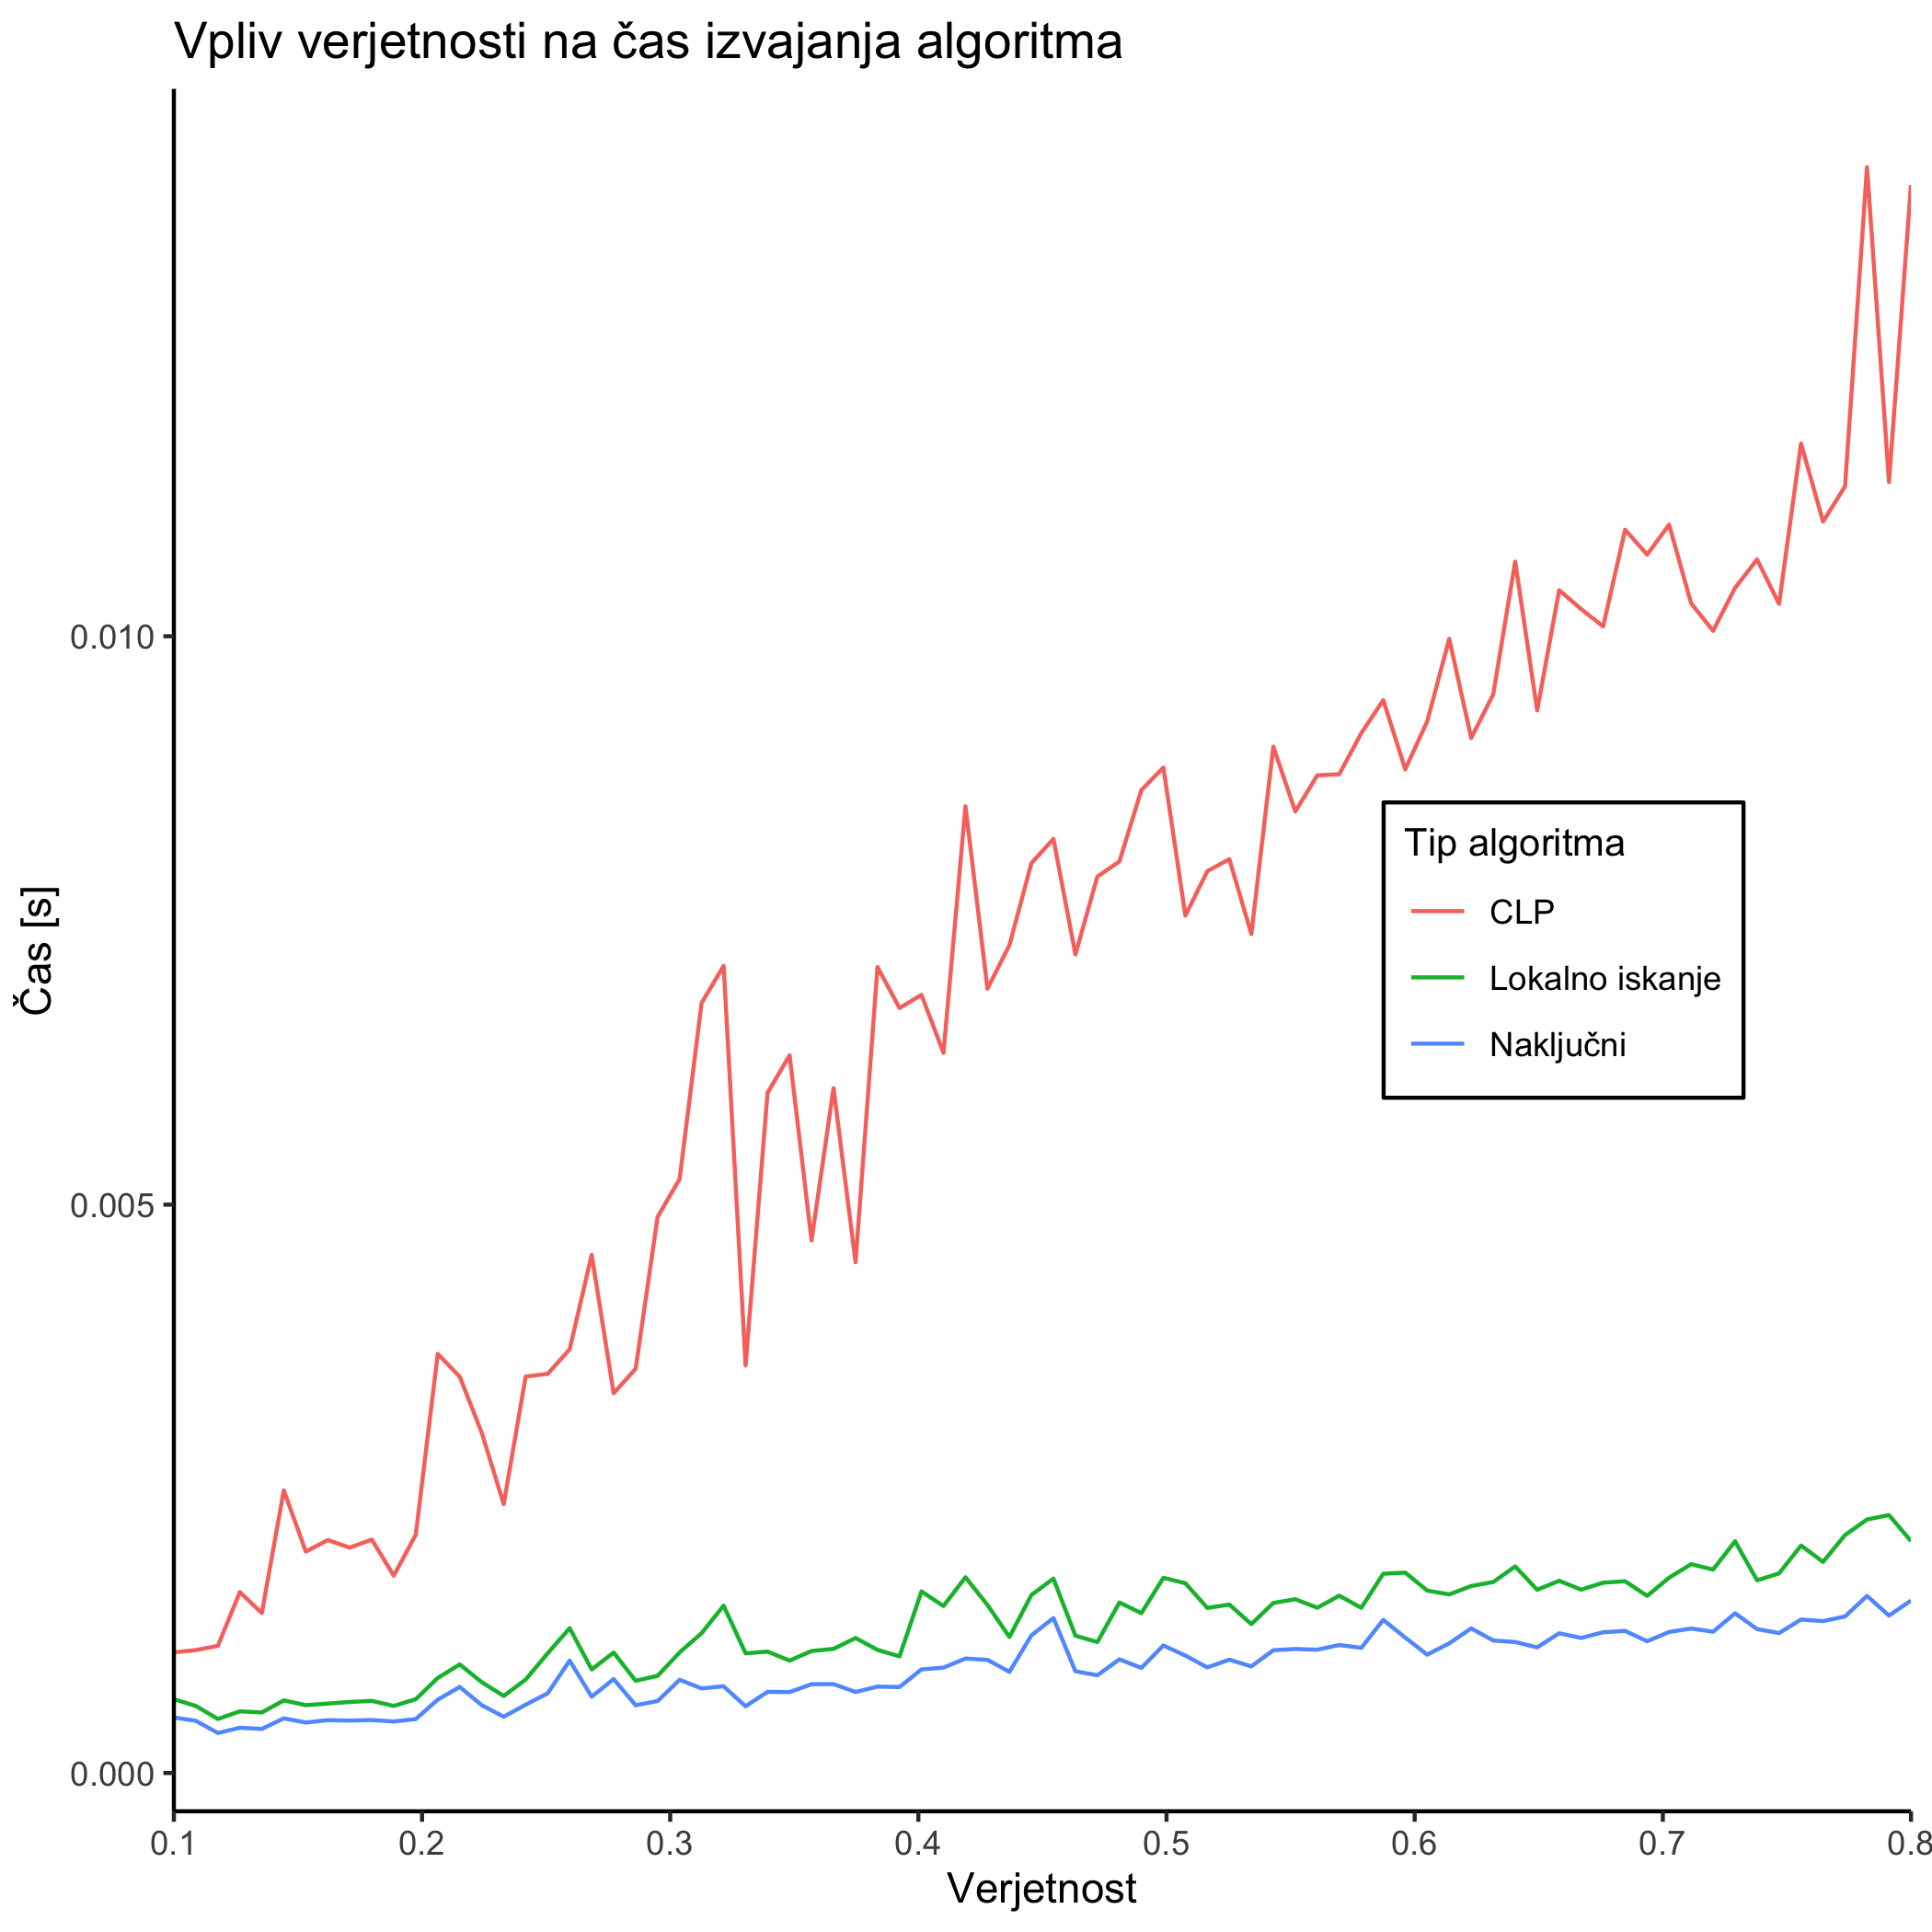
\includegraphics[scale=0.12]{R_koda/ver-cas.png}
		\caption{Vpliv verjetnosti na časovno zahtevnost algoritmov}
	\end{center}
\end{figure}


\newpage
\section{Zaključek}

Iz analize rezultatov lahko zaključimo, da v primeru generiranja grafov z \textit{Erdős-Rényijevim} $G(n, p)$ modelom, na velikost maksimalne neodvisne množice v danem grafu
vplivata tako število vozlišč v grafu, kot tudi število povezav. Kot alternativo iskanju maksimalne neodvisne množice s $CLP$-jem, sva uspela implementirati algoritem $nakljucni\_MIS$
in ga kasneje izboljšati z \textit{lokalnim\_iskanjem}. Čeprav so rešitve $CLP$ malenkost boljše v večini primerov, sta $nakljuci\_MIS$ in $lokalno\ iskanje$ boljša za grafe z večjim številom vozlišč,
ali pa z večjim številom povezav, saj sta manj časovno zahtevna.

\newpage

\begin{thebibliography}{9}    

    \bibitem{Mil} 
    Gary Miller.
    \textit{Lecture 32: Luby’s Algorithm for Maximal Independent Set}, dostopno na \url{http://www.cs.cmu.edu/afs/cs/academic/class/15750-s18/ScribeNotes/lecture32.pdf}.
    \bibitem{And, Res} 

    Diogo Andrade, Mauricio G. C. Resende.
    \textit{Fast Local Search for the Maximum Independent Set Problem.} Conference Paper in Journal of Heuristics, May 2008, 
    dostopno na \url{https://www.researchgate.net/publication/221131653_Fast_Local_Search_for_the_Maximum_Independent_Set_Problem}.

    \bibitem{Wiki} 
    \textit{Maximal independent set}, v: Wikipedia: The Free Encyclopedia,[ogled 6.~1.~2022], dostopno na \url{https://en.wikipedia.org/wiki/Maximal_independent_set}.

    \bibitem{Wiki} 
    \textit{Independent set (graph theory)}, v: Wikipedia: The Free Encyclopedia,[ogled 6.~1.~2022], dostopno na \url{https://en.wikipedia.org/wiki/Independent_set_(graph_theory)}.

    
\end{thebibliography}

\end{document}